\documentclass[a4paper,10pt]{article}
\usepackage[portuguese]{babel}

\usepackage{cite}
\usepackage{xcolor}
\usepackage{graphicx}
\usepackage{fancyhdr}
\usepackage[shortlabels]{enumitem}
\usepackage{amstext,amsmath,amssymb}

\usepackage{sectsty}
\sectionfont{\LARGE}

\setlength{\oddsidemargin}{0cm} %
\setlength{\evensidemargin}{0cm} %
\setlength{\topmargin}{0cm} %
\setlength{\textwidth}{16cm} %
\setlength{\textheight}{22.5cm} %

\pagestyle{empty}
\newcommand{\assunto}{Filtragem Adaptativa}

\sloppy

\begin{document}
	
	\thispagestyle{empty}

\begin{center}
  
    
\includegraphics[scale=0.10]{figs/icon.png}
    
    \LARGE{Universidade Federal do Ceará}
    
    \LARGE{Centro de Tecnologia}
    
    \LARGE{Departamento de Engenharia de Teleinformática}
    
    \LARGE{Engenharia de Teleinformática}
    
    \vspace{180pt}
      
    \LARGE{Filtragem Adaptativa}
      
    \LARGE{Listas de Exercícios Propostos}
      
    \vspace{100pt}
    
\end{center}

\vspace{25pt}

\begin{flushleft}
	\begin{tabbing}
		Student \qquad Kenneth Brenner dos Anjos Benício – 519189\\
	   \qquad\qquad\qquad\= \\
		Professor\> Charles Casimiro Cavalcante e Guilherme Barreto\\
		Course \> Filtragem Adaptativa - TIP7188\\
	\end{tabbing}
\end{flushleft}

\vspace{25pt}

\begin{center}
    Fortaleza, 2022
\end{center}
	
	\section*{Estatísticas de Segunda Ordem}
	
		\begin{enumerate}
			
			\item Determine a média e a função de autocorrelação para o processo aleatório em que $v(n)$ é uma sequência de variáveis aleatórias independentes com média $\mu$ e variância $\sigma^2$. $x(n)$ é estacionário? Justifique.
			
				\begin{align}
					&x(n) = v(n) + 3 v(n-1),
				\end{align}
				
				\textcolor{red}{Solução:}
				
				Para o cálculo da média é possível escrever
				
				\begin{align}
					&E[x(n)] = E[v(n) + 3v(n-1)], 
				\end{align}
				
				mas uma vez que todas as variáveis aleatórias possuem mesma média o resultado será
				
				\begin{align}
					&E[x(n)] = \mu + 3\mu = 4\mu.  
				\end{align}
				
				De forma semelhante a variância pode ser obtida por 
				
				\begin{align}
					&\mathbb{E}\{[(x(n) - \mu_{X})]^2\}, \\
					&\mathbb{E}\{[x(n) - 4\mu]^2\} = \mathbb{E}\{[v(n) - 3v(n-1) -4\mu]^{2}\}, \\
					&\mathbb{E}\{[x(n) - 4\mu]^2\} = \mathbb{E}\{[v(n) - \mu + 3v(n-1) -3\mu]^{2}\},
				\end{align}
				
				e ao desenvolver o valor quadrado da expressão chega-se em
				
				\begin{align}
					&\mathbb{E}\{[x(n) - 4\mu]^2\} = \mathbb{E}\{ [v(n) - \mu]^{2} + 9[v(n-1) - \mu]^{2} + 6[v(n) - \mu][v(n-1) - \mu] \}, \\
					&\mathbb{E}\{[x(n) - 4\mu]^2\} = \sigma^{2} + 9\sigma^{2} + \mathbb{E}\{6[v(n) - \mu][v(n-1) - \mu]\}.
				\end{align}
				
				Sabendo que os sinais são descorrelacionados uma vez que temos duas variáveis aleatórias independentes temos
				
				\begin{align}
					&6\mathbb{E}\{[v(n) - \mu][v(n-1) - \mu]\} = \mathbb{E}\{v(n)v(n-1) - \mu v(n) -\mu v(n-1) + \mu^{2}\}, \\
					&6\mathbb{E}\{[v(n) - \mu][v(n-1) - \mu]\} = \mathbb{E}\{v(n)v(n-1)\} - \mu^{2} -\mu^{2} + \mu^{2}, \\
					&6\mathbb{E}\{[v(n) - \mu][v(n-1) - \mu]\} = \mathbb{E}\{v(n)\} \mathbb{E}\{v(n-1)\} - \mu^{2}, \\
					&6\mathbb{E}\{[v(n) - \mu][v(n-1) - \mu]\} = \mu^{2} - \mu^{2} = 0,
				\end{align}
				
				Portanto, a média pode ser dada por
				
				\begin{align}
					&\mathbb{E}\{[x(n) - 4\mu]^2\} = 10\sigma^{2}. 
				\end{align}
				
				Além disso, a função de correlação pode ser adquirida por meio da seguinte operação 
				
				\begin{align}
					&\mathbb{E}\{x(n)x^{*}(n)\} = \mathbb{E}\{[v(n) + 3v(n-1)][v(n) + 3v(n-1)]^{*}\}, \\
					&\mathbb{E}\{x(n)x^{*}(n)\} = \mathbb{E}\{[v(n)v^{*}(n)] + 3[v(n)v^{*}(n-1)] + 3[v(n-1)v^{*}(n)] + [9v(n-1)v^{*}(n-1)]\},
				\end{align}
				
				onde é possível reescrever a equação acima ao considerarmos novamente a descorrelação entre as variáveis aleatórias 
				
				\begin{align}
					&\mathbb{E}\{x(n)x^{*}(n)\} = \mathbb{E}\{\mu^{2} + 3\mu^{2} + 3\mu^{2} + 9\mu^{2}\}, \\
					&\mathbb{E}\{x(n)x^{*}(n)\} = 16\mu^{2}.
				\end{align}
				
				Uma vez que as estatísticas de primeira e de segunda ordem são independentes quanto ao deslocamento temporal é possível afirmar que o processo descrito é Estacionário no Sentido Amplo(WSS). Entretanto, não é possível afirmar que o processo é Estacionário no Sentido Estrito(SSS) uma vez que não se tem conhecimento da função que descreve a densidade de probabilidade desse sistema.
			
			\item Sejam os processos aleatórios $x(n)$ e $y(n)$ definidos por
			
				\begin{align} 
					&x(n) = v_1(n) + 3v_2(n-1), \\
					&y(n) = v_2(n + 1) + 3v_1(n-1),
				\end{align}
				
				em que $v_1(n)$ e $v_2(n)$ são processos de ruído branco independentes cada um com variância igual a $0,5$.
				
				\begin{enumerate}
					
					\item Quais são as funções de autocorrelação de $x$ e de $y$? Os processos são WSS?
					
						\textcolor{red}{Solução:}
						
						Antes de tudo é de interesse definir o processo estocástico de ruído branco. Um processo desse tipo é formado por um número qualquer de amostras
						independentes entre si e com média nula. Desse modo, uma vez que a média de processos de ruído branco são nulas é possível obter facilmente a média dos novos processos formados pela combinação dos ruídos
						
						\begin{align}
							&\mathbb{E}\{x(n)\} = \mathbb{E}\{v_{1}(n) + 3v_{2}(n-1)\} = \mu_{1} + 3\mu_{2} = 0, \\
							&\mathbb{E}\{y(n)\} = \mathbb{E}\{v_{2}(n+1) + 3v_{1}(n-1)\} = \mu_{2} + 3\mu_{1} = 0.
						\end{align}
						
						Para a variância teremos uma resposta similar
						
						\begin{align*}
							&\mathbb{E}\{[x(n) - \mu]^{2}\} = \mathbb{E}\{[x(n) - 0]^{2}\} = \mathbb{E}\{[x(n)]^{2}\}, \\
							&\mathbb{E}\{[x(n) - \mu]^{2}\} = \mathbb{E}\{[v_{1}(n) + 3v_{2}(n-1)]^{2}\} = \mathbb{E}\{ [v^{2}_{1}(n)] + 6[v_{1}(n)v_{2}(n-1)] + 9[v^{2}_{2}(n-1)]\}, \\
							&\mathbb{E}\{[y(n) - \mu]^{2}\} = \mathbb{E}\{[y(n) - 0]^{2}\} = \mathbb{E}\{[y(n)]^{2}\}, \\
							&\mathbb{E}\{[y(n) - \mu]^{2}\} = \mathbb{E}\{[v_{2}(n+1) + 3v_{1}(n-1)]^{2}\} = \mathbb{E}\{ [v^{2}_{2}(n+1)] + 6[v_{2}(n+1)v_{1}(n-1)] + 9[v^{2}_{1}(n-1)]\}.
						\end{align*}
						
						Rescrevendo a expressão para obter a formula da variância e utilizando o fato dos processos de ruído serem descorrelacionados uma nova expressão é obtida
						
						\begin{align}
							&\mathbb{E}\{[x(n) - \mu]^{2}\} = \mathbb{E}\{ [v^{2}_{1}(n) - 0] + 0 + 9[v^{2}_{2}(n-1) - 0]\}, \\
							&\mathbb{E}\{[x(n) - \mu]^{2}\} = \sigma^{2}_{1} + 9\sigma^{2}_{2} = 10*0.5 = 5, \\
							&\mathbb{E}\{[y(n) - \mu]^{2}\} = \mathbb{E}\{ [v^{2}_{2}(n+1) - 0] + 0 + 9[v^{2}_{1}(n-1) - 0]\}, \\
							&\mathbb{E}\{[y(n) - \mu]^{2}\} = \sigma^{2}_{2} + 9\sigma^{2}_{1} = 10*0.5 = 5.
						\end{align}
						
						A função de autocorrelação para $X$ é calculada como se segue 
						\begin{align}
							r_{x}(\tau) &= \mathbb{E}\{x(n)x(n + \tau)\} = \mathbb{E}\{[v_{1}(n) + 3v_{2}(n-1)][v_{1}(n + \tau) + 3v_{2}(n-1 + \tau)]\}, \\
							r_{x}(\tau) &= \mathbb{E}\{[v_{1}(n)v_{1}(n + \tau)] + 3[v_{1}(n)v_{2}(n-1 + \tau)] + 3[v_{2}(n-1)v_{1}(n + \tau)] \\ 
							&+ 9[v_{2}(n-1)v_{2}(n-1 + \tau)] \}.    
						\end{align}
						
						Sabendo que amostras de um mesmo processo são descorrelacionadas e que ambos os processos também são descorrelacionados, além de termos conhecimento 
						de que ambos possuem média nula, então 
						
						\begin{align}
							&\mathbb{E}\{[v_{1}(n)v_{1}(n + \tau)]\} = \mathbb{E}\{[v_{1}(n)]\} \mathbb{E}\{[v_{1}(n + \tau)]\} = 0, \\ 
							&3\mathbb{E}\{[v_{1}(n)v_{2}(n-1 + \tau)]\} = 3\mathbb{E}\{[v_{1}(n)]\} \mathbb{E}\{[v_{2}(n-1 + \tau)]\} = 0, \\
							&3\mathbb{E}\{[v_{2}(n-1)v_{1}(n + \tau)]\} = 3\mathbb{E}\{[v_{2}(n-1)]\} \mathbb{E}\{[v_{1}(n + \tau)]\} = 0, \\
							&9\mathbb{E}\{[v_{2}(n-1)v_{2}(n-1 + \tau)]\} = 9\mathbb{E}\{[v_{2}(n-1)]\} \mathbb{E}\{[v_{2}(n-1 + \tau)]\} = 0, \\ 
							&r_{x}(\tau) = 0.
						\end{align}
						
						Repetindo o procedimento para $Y$ e omitindo informações redundantes chega-se ao seguinte resultado
						
						\begin{align}
							&r_{y}(\tau) = 0.
						\end{align}
						
						Sendo as estatísticas de primeira e de segunda ordem independentes quanto ao tempo para os dois processos então é possível afirmar que eles são WSS.
					
					\item Qual é a função de correlação cruzada $r_{xy}(n_1,n_0)$? Estes processos são conjuntamente estacionários (no sentido amplo)? Justifique.
					
						\textcolor{red}{Solução:}
						
						\begin{align}
							r_{x,y}(n_{1},n_{0}) &= \mathbb{E}\{[x(n_{1})y^{*}(n_{0})]\} = \mathbb{E}\{[v_{1}(n_{1}) + 3v_{2}(n_{1}-1)][v_{2}(n_{0}+1) + 3v_{1}(n_{0}-1)]^{*}\}, \\
							r_{x,y}(n_{1},n_{0}) &= \mathbb{E}\{[v_{1}(n_{1})v^{*}_{2}(n_{0}+1)] + 3[v_{1}(n_{1})v^{*}_{1}(n_{0}-1)] + 3[v_{2}(n_{1}-1)v^{*}_{2}(n_{0}+1)] \\ 
							&+ 9[v_{2}(n_{1}-1)v^{*}_{1}(n_{0}-1)]\}.  
						\end{align}
						
						Novamente considerando que os processos de ruído branco são descorrelacionadas entre si e que as amostras individuais são também independentes então podemos simplificar a expressão acima da seguinte forma
						
						\begin{align}
							&r_{x,y}(n_{1},n_{0}) = 0 
						\end{align}
						
						Sendo assim, os processos podem ser considerados conjuntamente estacionários uma vez que a correlação cruzada é independente do instante temporal e que os processos que compoem o processo conjunto podem 
						ser considerados estacionários em sentido amplo isoladamente. Entretanto, vale notar que foi possível realizar tal afirmação apenas por termos conhecimento da relação de independência entre os processos 
						de ruído branco, pois de outro modo não seria possível realizar afirmações quanto a correlação cruzada do processo conjunto.
					
				\end{enumerate}
			
			\item Quais as condições que os elementos de uma matriz
			
				\begin{align}
					\mathbf{R} = \left[
					\begin{matrix}
						a & b  \\
						c & d  \\
					\end{matrix} \right]
				\end{align}
				
				devem satisfazer tal que $\mathbf{R}$ seja uma matriz de autocorrelação válida de
			
				\begin{enumerate}
					
					\item Um vetor aleatório bidimensional?
					
						\textcolor{red}{Solução:}
						
						Em suma, precisamos estar atentos às seguintes propriedades para garantir que temos em mãos uma matriz de autocorrelação válida
						
						
						- $\mathbf{R_{x}} = \mathbf{R^{H}_{x}}$
						
						- $\mathbf{a^{H}} \mathbf{R_{xa}} \geq 0$
						
						- $\mathbf{Ax} = \lambda \mathbf{x}, \forall \lambda \geq 0 \text{ and } \mathbf{x} \in \mathbb{R}$
						
						Desse modo, considerando um vetor aleatório bidimensional descrito por $\mathbf{X} = (x_{1},x_{2})$ podemos então
						
						\begin{align}
							\mathbf{R} &= \left[ 
							\begin{matrix}
								\mathbb{E}\{[x^{2}_{1}]\} & \mathbb{E}\{[x_{1}x^{*}_{2}]\} \\
								\mathbb{E}\{[x_{2}x^{*}_{1}]\} & \mathbb{E}\{[x^{2}_{2}]\} \\
							\end{matrix} \right], \\
							\mathbf{R}^{\text{H}} &= \left[ 
							\begin{matrix}
								\mathbb{E}\{[x^{2}_{1}]\} & \mathbb{E}\{[x_{2}x^{*}_{1}]\} \\
								\mathbb{E}\{[x_{1}x^{*}_{2}]\} & \mathbb{E}\{[x^{2}_{2}]\} \\
							\end{matrix} \right].
						\end{align}
						
						Inicialmente, podemos garantir a simetria quanto ao hermitiano se fizermos 
						
						\begin{align}
							&\mathbb{E}\{[x_{1}x^{*}_{2}]\} \overset{\Delta}{=} \mathbb{E}\{[x_{2}x^{*}_{1}]\},
							&\mathbb{E}\{[x_{2}x^{*}_{1}]\} \overset{\Delta}{=} \mathbb{E}\{[x_{1}x^{*}_{2}]\}.
						\end{align}
						
						Entretanto, sabemos que o operador esperança é linear tornando assim as expressões acima equivalentes. Em continuidade do problema, podemos 
						considerar que a restrição as quais os autovalores estão submetidos pode ser facilmente atingida ao garantirmos que o determinante da matriz 
						de correlação seja maior que a nulidade
						
						\begin{align}
							&\mathbb{E}\{[x^{2}_{1}]\} \mathbb{E}\{[x^{2}_{1}]\} - \mathbb{E}\{[x_{1}x_{2}]\} \mathbb{E}\{[x_{2}x_{1}]\} > 0, \\
							&\mathbb{E}\{[x_{1}^{2}]\} \mathbb{E}\{[x^{2}_{2}]\} > \mathbb{E}\{[x_{1}x_{2}]\} \mathbb{E}\{[x_{2}x_{1}]\}.
						\end{align}
				
					\item Um processo estocástico estacionário escalar?
					
						\textcolor{red}{Solução:}
						
						Considerando um processo estocástico estacionário escalar do tipo $\mathbf{X}_{t} = x(t)$ e uma versão atrasada desse
						processo definida por $\mathbf{X}_{t + \tau} = x(t + \tau)$ temos que a matriz de correlação pode ser escrita da seguinte forma
						
						\begin{align}
							\mathbf{R} &= \left[ 
							\begin{matrix}
								\mathbb{E}\{[x^{2}(t)_{1}]\} & \mathbb{E}\{[x(t)x^{*}(t + \tau)]\} \\
								\mathbb{E}\{[x(t + \tau)x^{*}(t)]\} & \mathbb{E}\{[x^{2}(t + \tau)]\} \\
							\end{matrix} \right], \\
							\mathbf{R}^{\text{H}} &= \left[ 
							\begin{matrix}
								\mathbb{E}\{[x^{2}(t)_{1}]\} & \mathbb{E}\{[x(t + \tau)x^{*}(t)]\} \\
								\mathbb{E}\{[x(t)x^{*}(t + \tau)]\} & \mathbb{E}\{[x^{2}(t + \tau)]\} \\
							\end{matrix} \right].
						\end{align}
						
						
						Em sequência, podemos garantir a simetria quanto ao hermitiano se fizermos 
						
						\begin{align}
							&\mathbb{E}\{[x(t)x^{*}(t + \tau)]\} \overset{\Delta}{=} \mathbb{E}\{[x(t + \tau)x^{*}(t)]\}, \\
							&\mathbb{E}\{[x(t + \tau)x^{*}(t)]\} \overset{\Delta}{=} \mathbb{E}\{[x(t)x^{*}(t + \tau)]\},
						\end{align}
						
						mas, mais uma vez, considerando que o operador esperança é linear então as duas expressões são equivalentes. Já considerando a
						restrição imposta aos autovalores da matriz temos novamente
						
						\begin{align}
							&\mathbb{E}\{[x^{2}(t)]\} \mathbb{E}\{[x^{2}(t + \tau)]\} > \mathbb{E}\{[x(t)x^{*}(t + \tau)]]\}  \mathbb{E}\{[x(t + \tau)]x^{*}(t)]\}.
						\end{align}
					
				\end{enumerate}
			
			\item Assuma que a inversa $\mathbf{R}_{\mathbf{x}}^{-1}$ da matriz de autocorrelação de um vetor coluna $N$-dimensional exista. Mostre que
			
				\begin{align}
					\mathbb{E}\left\{\mathbf{x}^H \mathbf{R}_{\mathbf{x}}^{-1} \mathbf{x} \right\} = N
				\end{align}
				
				\textcolor{red}{Solução:}
				
				Inicialmente podemos escrever a expressão regular para a matriz de autocorrelação e supondo que de fato existe uma inversa bem definida 
				para a matriz de autocorrelação
				
				\begin{align}
					\mathbb{E}\{\mathbf{x} \mathbf{x}^{\text{H}}\} = \mathbf{R}_{x}, \\
					\mathbb{E}\{\mathbf{x} \mathbf{x}^{\text{H}}\}\mathbf{R}^{-1}_{x} = \mathbf{R}_{x}\mathbf{R}^{-1}_{x}, \\
					\mathbb{E}\{\mathbf{x} \mathbf{x}^{\text{H}}\mathbf{R}^{-1}_{x}\} = \mathbf{I}_{N}, \\
				\end{align}
				
				Desse modo, podemos aplicar o operador traço de matriz e por meio da propriedade de permutação cíclica desse operador chegamos ao seguinte resultado
				
				\begin{align}
					\text{Tr}\{\mathbb{E}\{\mathbf{x} \mathbf{x}^{\text{H}}\mathbf{R}^{-1}_{x}\}\} = \text{Tr}\{\mathbf{I}_{N}\}, \\
					\text{Tr}\{\mathbb{E}\{\mathbf{x}^{\text{H}}\mathbf{R}^{-1}_{x} \mathbf{x}\}\} = \text{Tr}\{\mathbf{I}_{N}\}, \\
					\text{Tr}\{\mathbb{E}\{\mathbf{x}^{\text{H}}\mathbf{R}^{-1}_{x} \mathbf{x}\}\} = N,
				\end{align}
			
				onde a ultima expressão se justifica pois temos uma matriz identidade de ordem $N$ no lado direito. Desse modo, seu traço é dado por $\sum^{N}_{i = 1} 1 = N$.
				
			\item Mostre que as matrizes de correlação e covariância satisfazem as relações abaixo:
				
				\begin{enumerate}
					
					\item $\mathbf{R}_\mathbf{x} = \mathbf{C}_\mathbf{x} + {\mathbf{\mu}}_{\mathbf{x}}{\mathbf{\mu}}_{\mathbf{x}}^H$
					
						\textcolor{red}{Solução:}
						
						\begin{align}
							&C_{X} = \mathbb{E}\{[(x - \mu)(x - \mu)^{H}]\} = \mathbb{E}\{[xx^{H} -x\mu^{H} - \mu x^{H} + \mu \mu^{H}]\}, \\
							&C_{X} = \mathbb{E}\{[xx^{H}]\} -\mathbb{E}\{[x\mu^{H}]\} - \mathbb{E}\{[\mu x^{H}]\} + \mathbb{E}\{[\mu \mu^{H}]\}.
						\end{align}
						
						
						Considerando a matriz de correlação pode ser escrita por $R_{X} = \mathbb{E}\{[xx^{H}]\}$ e que o valor médio de um escalar é o próprio escalar temos
						
						\begin{align}
							&C_{X} = R_{X} - \mathbb{E}\{[x\mu^{H}]\} - \mathbb{E}\{[\mu x^{H}]\} + \mu \mu^{H}, \\
							&C_{X} = R_{X} - \mu^{H}\mathbb{E}\{[x]\} - \mu \mathbb{E}\{[x^{H}]\} + \mu \mu^{H}, \\
							&C_{X} = R_{X} - \mu \mu^{H} - \mu \mu^{H} + \mu \mu^{H}, \\
							&C_{X} = R_{X} - \mu \mu^{H}, \\
							&R_{X} = C_{X} + \mu \mu^{H}.
						\end{align}
					
					\item $\mathbf{C}_{\mathbf{x} + \mathbf{y}} = \mathbf{C}_{\mathbf{x}} +
					\mathbf{C}_{\mathbf{y}}$, para $\mathbf{x}$ e $\mathbf{y}$ descorrelacionados
					
						\textcolor{red}{Solução:}
						
						\begin{align}
							&\mathbf{C}_{\mathbf{x} + \mathbf{y}} = \mathbf{C}_{\mathbf{x}} + \mathbf{C}_{\mathbf{xy}} + \mathbf{C}_{\mathbf{yx}} + \mathbf{C}_{\mathbf{y}}.
						\end{align}
						
						Onde os termos de correlação cruzada $\mathbf{C}_{\mathbf{xy}}$ e $\mathbf{C}_{\mathbf{yx}}$ podem ser obtidos  da seguinte maneira
						
						\begin{align}
							&\mathbf{C_{xy}} = \mathbb{E}\{[x - \mu_{x}][y - \mu_{y}]\}, \\
							&\mathbf{C_{xy}} = \mathbb{E}\{[xy]\} - \mathbb{E}\{[x\mu_{y}]\} - \mathbb{E}\{[\mu_{x} y]\} + \mathbb{E}\{[\mu_{x} \mu_{y}]\}, \\
							&\mathbf{C_{xy}} = \mathbb{E}\{[xy]\} - \mu_{y} \mu_{x} - \mu_{x} \mu_{y} + \mu_{x} \mu_{y}, \\
							&\mathbf{C_{xy}} = \mathbb{E}\{[xy]\} + \mu_{x} \mu_{y}, \\
							&\mathbf{C_{xy}} = \mu_{x} \mu_{y}, \\
						\end{align}
						
						\begin{align}
							&\mathbf{C_{yx}} = \mathbb{E}\{[y - \mu_{y}][x - \mu_{x}]\}, \\
							&\mathbf{C_{yx}} = \mathbb{E}\{[yx]\} - \mathbb{E}\{[y\mu_{x}]\} - \mathbb{E}\{[\mu_{y} x]\} + \mathbb{E}\{[\mu_{y} \mu_{x}]\}, \\
							&\mathbf{C_{yx}} = \mathbb{E}\{[yx]\} - \mu_{y} \mu_{x} - \mu_{x} \mu_{y} + \mu_{y} \mu_{x}, \\
							&\mathbf{C_{yx}} = \mathbb{E}\{[yx]\} - \mu_{x} \mu_{y}, \\
							&\mathbf{C_{yx}} = - \mu_{x} \mu_{y}.
						\end{align}
						
						Portanto, é possível afirmar que a soma dos termos de correlação cruzada é nula e que a correlação da soma de dois vetores descorrelacionados é de fato 
						dada por $\mathbf{C}_{\mathbf{x} + \mathbf{y}} = \mathbf{C}_{\mathbf{x}} + \mathbf{C}_{\mathbf{y}}$
						
						\begin{align}
							&\mathbf{C_{xy}} + \mathbf{C_{yx}}  = \mu_{x} \mu_{y} - \mu_{x} \mu_{y}, \\
							&\mathbf{C_{xy}} + \mathbf{C_{yx}}  = 0.
						\end{align}
					
					
				\end{enumerate}
			
			\item Processos aleatórios $v_1(n)$ e $v_2(n)$  são independentes e têm a mesma função de correlação
			
				\begin{align}
					r_v(n_1,n_0) = 0.5\delta(n_1 - n_0)
				\end{align}
			 
			 	\begin{enumerate}
			 		
			 		\item Qual é a função de correlação do processo aleatório
			 		
				 		\begin{align}
				 			x(n) = v_1(n) + 2v_1(n + 1) + 3v_2(n-1) ?
				 		\end{align}
				 		
				 		Este é um processo WSS? Justifique.
				 		
				 		\textcolor{red}{Solução:}
				 		
				 		Para simplificar o desenvolvimento iremos considerar que os processos possuem media nula e são descorrelacionados
				 		
				 		\begin{align*}
				 			r_{x} &= \mathbb{E}\{x(n) x^{*}(n)\}, \\
				 			r_{x} &= \mathbb{E}\{[v_{1}(n) + 2v_{1}(n+1) + 3v_{2}(n-1)] [v_{1}(n) + 2v_{1}(n+1) + 3v_{2}(n-1)]^{*}(n)\}, \\
				 			r_{x} &= \mathbb{E}\{[v_{1}(n)v^{*}_{1}(n) + 2v_{1}(n)v^{*}_{1}(n+1) + 3v_{1}(n)v^{*}_{2}(n-1) + 2v_{1}(n + 1)v^{*}_{1}(n) + 4v_{1}(n+1)v^{*}_{1}(n+1) \\
							&+6v_{1}(n+1)v^{*}_{2}(n-1)] + 3v_{2}(n-1)v^{*}_{1}(n) +  6v_{2}(n-1)v^{*}_{1}(n+1) + 9v_{2}(n-1)v^{*}_{2}(n-1)\}, \\
				 			r_{x} &= r_{v}(n,n) + 2r_{v}(n,n+1) + 0 + 2r_{v}(n+1,n) + 4r_{v}(n+1,n+1) + 0 + 0 + 0 + 9r_{v}(n-1,n-1), \\
				 			r_{x} &= r_{v}(n,n) + 2r_{v}(n,n+1) + 2r_{v}(n+1,n) + 4r_{v}(n+1,n+1) + 9r_{v}(n-1,n-1).
				 		\end{align*}
				 		
				 		Após uma breve análise na expressão $r_{v}(n_{1},n_{0})$ é possível verificar que determinados termos anulam-se ao considerar um único momento temporal devido a presença da função degrau unitário, permitindo a seguinte simplificação:
				 		
				 		\begin{align}
				 			&r_{x} = 2r_{v}(n,n+1) + 2r_{v}(n+1,n), \\
				 			&r_{x} = \delta(n - n - 1) + \delta(n + 1 - n).
				 		\end{align}
				 		
				 		Onde a generalização pode ser descrita por:
				 		
				 		\begin{align}
				 			&r_{x}(n_{1}, n_{2})= \delta(n_{1} - n_{2}) + \delta(n_{2} - n_{1}).  
				 		\end{align}
				 		
				 		Uma vez que a correlação é dependente apenas de um deslocamento temporal, então podemos classificar esse processo como WSS.
			 		
			 		\item Encontre a a matrix de correlação de um vetor aleatório consistindo de oito amostras consecutivas de
			 		$x(n)$.
			 		
				 		\textcolor{red}{Solução:}
				 		
				 		\begin{align}
				 			\mathbf{R}_{\mathbf{x}} = \left[
				 			\begin{matrix}
				 				2 & 0 & 0 & 0 & 0 & 0 & 0 & 0\\
				 				0 & 2 & 0 & 0 & 0 & 0 & 0 & 0\\
				 				0 & 0 & 2 & 0 & 0 & 0 & 0 & 0\\
				 				0 & 0 & 0 & 2 & 0 & 0 & 0 & 0\\
				 				0 & 0 & 0 & 0 & 2 & 0 & 0 & 0\\
				 				0 & 0 & 0 & 0 & 0 & 2 & 0 & 0\\
				 				0 & 0 & 0 & 0 & 0 & 0 & 2 & 0\\
				 				0 & 0 & 0 & 0 & 0 & 0 & 0 & 2
				 			\end{matrix}
				 			\right]
				 		\end{align}
				 		
				 		Para chegar a esse resultado foi utilizado a expressão para a correlação obtida no item anterior. Uma vez que a função delta de dirac terá um valor não nulo apenas quando o argumento for zero, isso irá acontecer apenas quando os momentos $n_{1}$ e $n_{2}$ forem iguais e isso irá acontecer apenas com os elementos da diagonal principal.
			 		
			 	\end{enumerate}
		 	
		\end{enumerate}
		
	\newpage
	\section*{Filtragem Linear Ótima}
	
		\begin{enumerate}
			
			\item Considere um problema de filtragem de Wiener conforme caracterizado a seguir. A matriz de correlação $\mathbf{R}_{\mathbf{x}}$ de um vetor de entrada $\mathbf{x}(n)$ é dada por
			
				\begin{align*}
					\mathbf{R}_{\mathbf{x}} = \left[ \begin{matrix}
						1 & {0.5}  \\   {0.5} & 1  \\ \end{matrix} \right].
				\end{align*}
				
				O vetor de correlação cruzada $\mathbf{p}_{\mathbf{x}d}$ entre o vetor de entrada $\mathbf{x}$ e a resposta desejada
				$d(n)$ é
				
				\begin{align*}
					\mathbf{p}_{\mathbf{x}d} &= \left[ \begin{matrix}   {0.5}  \\   {0.25}  \\ \end{matrix} \right]
				\end{align*}
				
				\begin{enumerate}
					
					\item Encontre o vetor de coeficientes do filtro de Wiener.
					
						\textcolor{red}{Solução:}
						
						Isso pode ser realizado de forma simples pelo uso da equação do filtro ótimo de wiener
						
						\begin{align}
							\mathbf{w}_{\text{opt}} &= \mathbf{R}^{-1}_{X} \mathbf{p}_{xd}, \\
							\mathbf{w}_{\text{opt}} &=  \left[ \begin{matrix} 1 & 0.5 \\ 0.5 & 1 \end{matrix} \right]  \left[ \begin{matrix} 0.5 \\ 0.25 \end{matrix} \right], \\
							\mathbf{w}_{\text{opt}} &=  \frac{4}{3} \left[ \begin{matrix} 1 & -0.5 \\ -0.5 & 1 \end{matrix} \right]  \left[ \begin{matrix} 0.5 \\ 0.25 \end{matrix} \right], \\
							\mathbf{w}_{\text{opt}} &= \left[ \begin{matrix} 0.5 \\ 0.0 \end{matrix} \right].
						\end{align}
					
					\item Qual é o mínimo erro médio quadrático fornecido por este filtro?
					
						\textcolor{red}{Solução:}
						
						\begin{align}
							\mathbb{E}\{e^{2}(n)\}  &=\sigma^{2}_{d} - 2\mathbf{w}^{T}\mathbf{p}_{xd} + w^{T}\mathbf{R}_{X}\mathbf{w}      
						\end{align}
						
						Ao aplicar o vetor descoberto no item anterior obtem-se o erro mínimo
						
						\begin{align}
							e_{min}  &=\sigma^{2}_{d} - 2\mathbf{w}^{T}_{opt}\mathbf{p}_{xd} + w^{T}_{opt}\mathbf{R}_{X}\mathbf{w}_{\text{opt}}, \\
							e_{min} &= \sigma^{2}_{d} - 2 \left[ \begin{matrix} 0.5 & 0.0 \end{matrix} \right] \left[ \begin{matrix} 0.5 \\ 0.25 \end{matrix} \right] + \left[ \begin{matrix} 0.5 & 0.0 \end{matrix} \right] \left[ \begin{matrix} 1 & -0.5 \\ -0.5 & 1 \end{matrix} \right]  \left[ \begin{matrix} 0.5  \\ 0.0 \end{matrix} \right], \\
							e_{min} &= \sigma^{2}_{d} - 2 * 0.25 + 0.25, \\
							e_{min} &= \sigma^{2}_{d} - 0.25. 
						\end{align}
						
						Dessa forma o erro é dependente da variância do sinal desejado.					
					
					\item Formule uma representação do filtro de Wiener em termos dos autovalores da matriz $\mathbf{R}_{\mathbf{x}}$
					e de seus autovetores associados.
					
						\textcolor{red}{Solução:}
						
						Utilizando a decomposição matricial em autovalores (EVD) é possível reescrever a matrix de correlação como abaixo
						
						\begin{align}
							\mathbf{R}_{X} &= \mathbf{Q} \mathbf{\Lambda} \mathbf{Q}^{-1}.
						\end{align}
						
						A matriz $\mathbf{\Lambda}$ contémm os autovalores $\lambda_{i}$ e a matriz $\mathbf{Q}$ os respectivos autovetores. Em posse dessa relação é possível reescrever a equação do fitro ótimo de wiener como
						
						\begin{align}
							\mathbf{w}_{\text{opt}} &= \mathbf{R}^{-1}_{X} \mathbf{p}_{xd}, \\
							\mathbf{w}_{\text{opt}} &= (\mathbf{Q} \mathbf{\Lambda} \mathbf{Q}^{-1})^{-1} \mathbf{p}_{xd}, \\
							\mathbf{w}_{\text{opt}} &= \mathbf{Q}^{-1} \mathbf{\Lambda}^{-1} \mathbf{Q} \mathbf{p}_{xd}.
						\end{align}
						
						É possível verificar de imediato que essa propriedade é bem útil uma vez que a inversa de uma matriz diagonal é certamente menos custosa que a inversa da matriz de autocorrelação completa.
					
				\end{enumerate}
			
			\item Mostre que a equação do erro mínimo pode se escrita da seguinte maneira
			
				\begin{align*}
					\mathbf{A}\left[ \begin{matrix}
						1  \\
						{ - \mathbf{w}}  \\
					\end{matrix} \right] = \left[ \begin{matrix}
						J_{\text{min}}  \\
						\mathbf{0}  \\
					\end{matrix} \right],
				\end{align*}
				
				em que $J_{\text{min}}$ é o mínimo erro médio quadrático, $\mathbf{w}$ é o filtro de Wiener, e $\mathbf{A}$ é a matriz de
				correlação do vetor aumentado
				
				\begin{align*}
					\left[ \begin{matrix}
						d(n)  \\
						\mathbf{x}(n)  \\
					\end{matrix} \right],
				\end{align*}
				
				em que $d(n)$ é o sinal desejado e $\mathbf{x(n)}$ é o sinal de entrada do filtro de Wiener.
				
				\textcolor{red}{Solução:}
				
				Inicialmente deve-se calcular a matriz de correlação do vetor aumentado
				
				\begin{align}
					\mathbf{A} &= \mathbb{E} \{ \left[ \begin{matrix} d(n) \\ x(n) \end{matrix} \right] \left[ \begin{matrix} d(n)^{T} & x(n)^{T} \end{matrix} \right] \}, \\
					\mathbf{A} &=   \left[ \begin{matrix} \mathbb{E}\{d(n) d(n)^{T}\} & \mathbb{E}\{d(n) x(n)^{T}\} \\ \mathbb{E}\{x(n) d(n)^{T}\} & \mathbb{E}\{x(n) x(n)^{T}\} \end{matrix} \right].
				\end{align}
				
				Dando as devidas nomeações aos termos a expressão acima reduz-se a
				
				\begin{align}
					\mathbf{A} &=  \left[ \begin{matrix} \sigma^{2}_{d} & \mathbf{p}_{xd}^{T} \\
						\mathbf{p}_{xd} & \mathbf{R}_{X} \end{matrix} \right].
				\end{align}
				
				Multiplicando-se a expressão acima pelo vetor $[1 - \mathbf{w}]^{T}$
				
				\begin{align}
					\mathbf{A} \left[ \begin{matrix} 1 \\ -\mathbf{w} \end{matrix} \right] &=   \left[ \begin{matrix} \sigma^{2}_{d} & \mathbf{p}_{xd}^{T} \\
						\mathbf{p}_{xd} & \mathbf{R}_{X} \end{matrix} \right] \left[ \begin{matrix} 1 \\ -\mathbf{w} \end{matrix} \right], \\
					\mathbf{A} \left[ \begin{matrix} 1 \\ -\mathbf{w} \end{matrix} \right] &=   \left[ \begin{matrix} \sigma^{2}_{d} - \mathbf{p}_{xd}^{T}\mathbf{w} \\
						\mathbf{p}_{xd} - \mathbf{R}_{X}\mathbf{w} \end{matrix} \right].
				\end{align}
				
				Por fim, resta apenas aplica a equação ótima do filtro de wiener $\mathbf{w}_{\text{opt}} = \mathbf{R}^{-1}_{X} \mathbf{p}_{xd}$
				
				\begin{align}
					\mathbf{A} \left[ \begin{matrix} 1 \\ -\mathbf{w} \end{matrix} \right] &=   \left[ \begin{matrix} \sigma^{2}_{d} - \mathbf{p}_{xd}^{T}\mathbf{R}^{-1}_{X} \mathbf{p}_{xd} \\
						\mathbf{p}_{xd} - \mathbf{R}_{X}\mathbf{R}^{-1}_{X} \mathbf{p}_{xd} \end{matrix} \right], \\
					\mathbf{A} \left[ \begin{matrix} 1 \\ -\mathbf{w} \end{matrix} \right] &=   \left[ \begin{matrix} \sigma^{2}_{d} - \mathbf{p}_{xd}^{T}\mathbf{R}^{-1}_{X} \mathbf{p}_{xd} \\
						\mathbf{p}_{xd} - \mathbf{I}_{X}\mathbf{p}_{xd} \end{matrix} \right], \\
					\mathbf{A} \left[ \begin{matrix} 1 \\ -\mathbf{w} \end{matrix} \right] &=   \left[ \begin{matrix} \sigma^{2}_{d} - \mathbf{p}_{xd}^{T
						}\mathbf{R}^{-1}_{X} \mathbf{p}_{xd} \\ 0 \end{matrix} \right], \\
					\mathbf{A} \left[ \begin{matrix} 1 \\ -\mathbf{w} \end{matrix} \right] &=   \left[ \begin{matrix} J_{min} \\ 0 \end{matrix} \right].
				\end{align}
			
			\item Em várias aplicações práticas há uma necessidade de cancelar ruído que foi adicionado a um sinal. Por exemplo, se estamos usando o telefone celular dentro de um ruído e o ruído do carro ou rádio é adicionado à mensagem que estamos tentando transmitir. A Figura abaixo ilustra as situações de contaminação de ruído. Calcule o filtro de Wiener (filtro ótimo) de tal configuração em relação às estatísticas dos sinais envolvidos que você dispõe (conhece).
			
				\begin{figure}[!ht]
					\centering
					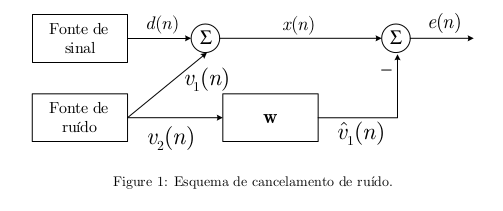
\includegraphics[width=0.5\textwidth]{figs/cancelamento_ruido.png}
					\caption{Estrutura de Equalização de Canal}
				\end{figure}
				
				\textcolor{red}{Solução:}
				
				Inicialmente é necessário calcular a equação de erro do sistema aqui proposto
				
				\begin{align}
					e(n) &= x(n) - \hat{v_{1}} = x(n) - \mathbf{w}^{T}v_{2}(n)
				\end{align}
				
				Em seguida faz-necessário calcular a função mean square error(MSE) que é facilmente fornecida pela manipulação algébrica abaixo
				
				\begin{align}
					e^{2}(n) &= [x(n) - \mathbf{w}^{T}v_{2}(n)][x(n) - \mathbf{w}^{T}v_{2}(n)]^{T}, \\
					e^{2}(n) &= x^{2}(n) - 2x(n)\mathbf{w}^{T}v_{2}(n) + \mathbf{w}^{T}v_{2}(n)v_{2}^{T}\mathbf{w}.
				\end{align}
				
				Sendo considerado que o filtro apresenta coeficientes constantes é possível aplicar o operador Valor Esperado de forma a obter a seguinte relação
				
				\begin{align}
					\mathbb{E}\{e^{2}(n)\} = \mathbb{E}\{x^{2}(n)\} - 2\mathbf{w}^{T}\mathbb{E}\{x(n) v_{2}(n)\} + \mathbf{w}^{T}\mathbb{E}\{v_{2}(n)v_{2}(n)^{T}\} \mathbf{w},& \\
					\mathbb{E}\{e^{2}(n)\} = \sigma^{2}_{x} - 2\mathbf{w}^{T}\mathbf{p}_{xv_{2}} + \mathbf{w}^{T}\mathbf{R}_{v_{2}} \mathbf{w}.&
				\end{align}
				
				Por fim, basta encontrar o $\mathbf{w}$ que minimiza o MSE acima. Para chegar a esse fim, calcula-se o gradiante quanto ao $\mathbf{w}$ igualando-se o resultado da operação a zero
				
				\begin{align}
					\nabla_{\mathbf{w}} \mathbb{E}\{e^{2}(n)\} = - 2\mathbf{p}_{xv_{2}} + 2\mathbf{R}_{v_{2}} \mathbf{w} = 0,& \\
					-\mathbf{p}_{xv_{2}} + \mathbf{R}_{v_{2}} \mathbf{w} = 0,& \\
					\mathbf{R}_{v_{2}} \mathbf{w} = \mathbf{p}_{xv_{2}}.&
				\end{align}
				
				Utilizando a identidade matricial abaixo é possível resolver a equação acima para obter o seguinte resultado
				
				\begin{align}
					\mathbf{R}^{-1}_{v_{2}}\mathbf{R}_{v_{2}} \mathbf{w} &= \mathbf{R}^{-1}_{v_{2}}\mathbf{p}_{xv_{2}}, \\
					\mathbf{I}\mathbf{w} &= \mathbf{R}^{-1}_{v_{2}}\mathbf{p}_{xv_{2}}, \\ 
					\mathbf{w} &= \mathbf{R}^{-1}_{v_{2}}\mathbf{p}_{xv_{2}}. 
				\end{align}
				
				Onde é possível reescrever o termo final como
				
				\begin{align}
					\mathbf{w} = \mathbf{R}^{-1}_{v_{2}}(\mathbf{p}_{d} + \mathbf{p}_{v_{1}} + \mathbf{p}_{v_{2}}) 
				\end{align}
			
			\item Seja um processo estocástico dado pela expressão abaixo onde $S(n)$ é um processo estocástico WSS dado e $a$ é uma constante.
			
				\begin{align*}
					x(n) = s(n + a) + s(n-4a),
				\end{align*}
				
				Deseja-se filtrar o processo de tal forma obter-se um processo $D(s) = s(n -a)$, o qual também sabe-se que é um processo WSS. Suponha que o sinal $d(n)$ possua média nula e variância unitária.
			
				\begin{enumerate}
					
					\item Calcule o filtro, com dois coeficientes, que fornece a solução ótima em relação ao erro médio quadrático.
					
						\textcolor{red}{Solução:}

						O filtro linear ótimo que minimiza o erro médio quadrático é descrito pela solução das equações de Wiener. Portanto, inicialmente definir a matriz de autocorrelação para o processo descrito por $x(n)$

						\begin{align} 
							\mathbf{R}_{x} = 
							\begin{bmatrix}
								\mathbb{E}\{x(n)x^{*}(n)\} & \mathbb{E}\{x(n-1)x^{*}(n)\} \\
								\mathbb{E}\{x(n)x^{*}(n-1)\}  & \mathbb{E}\{x(n-1)x^{*}(n-1)\} 
							\end{bmatrix},
						\end{align}
					
						se considerarmos que o processo $S(n)$ é WSS com variância $\sigma^{2}_{s}$ podemos calcular as correlações como se segue

						\begin{align*} 
							\mathbb{E}\{x(n)x^{*}(n)\} &= \mathbb{E}\{ s(n - a) s^{*}(n - a) + s(n - a) s^{*}(n - 4a) + s(n - 4a) s^{*}(n - a) \\
							&+ s(n - 4a) s^{*}(n - 4a) \} = \sigma^{2}_{s} + 0 + 0 + \sigma^{2}_{s} = 2\sigma^{2}_{s} , \\
							\mathbb{E}\{x(n-1)x^{*}(n)\} &= \mathbb{E}\{ s(n - 1 -a) s^{*}(n - a) + s(n - 1 - a) s^{*}(n - 4a) + s(n - 1 - 4a) s^{*}(n - a) \\
							&+ s(n - 1 - 4a) s^{*}(n - 4a) \} = 0 + 0 + 0 + 0 = 0, \\
							\mathbb{E}\{x(n)x^{*}(n-1)\} &= \mathbb{E}\{ s(n - a) s^{*}(n - 1 - a) + s(n - a) s^{*}(n - 1 - 4a) + s(n - 4a) s^{*}(n - 1 - a) \\
							&+ s(n - 4a) s^{*}(n - 1 - 4a) \} = 0 + 0 + 0 + 0 = 0, \\
							\mathbb{E}\{x(n-1)x^{*}(n-1)\} &= \mathbb{E}\{ s(n - 1 -a) s^{*}(n - 1 - a) + s(n - 1 - a) s^{*}(n - 1 - 4a) \\
							&+ s(n - 1 - 4a) s^{*}(n - 1 - a) + s(n - 1 - 4a) s^{*}(n - 1 - 4a) \} = \sigma^{2}_{s} + 0 + 0 + \sigma^{2}_{s} = 2\sigma^{2}_{s}, \\
						\end{align*}

						obtendo assim
						
						\begin{align} 
							\mathbf{R}_{x} = 
							\begin{bmatrix}
								2 \sigma^{2}_{s} & 0 \\
								0  & 2 \sigma^{2}_{s}
							\end{bmatrix},
						\end{align}

						Entretanto, considerando que o processo $D(n)$ têm média nula então temos na verdade um vetor de correlação cruzada nulo. Desse modo, o filtro linear
						ótimo para esse processo seria o próprio vetor nulo. Sendo assim

						\begin{align} 
							\mathbf{w}_{\text{opt}} = \mathbf{R}^{-1}_{x} \mathbf{p}_{xd} = 
							\begin{bmatrix}
								2 \sigma^{2}_{s} & 0 \\
								0  & 2 \sigma^{2}_{s}
							\end{bmatrix}
							\begin{bmatrix}
								0 \\
								0 
							\end{bmatrix} = 
							\begin{bmatrix}
								0 \\
								0 
							\end{bmatrix},  
						\end{align}
						


					\item Calcule o preditor direto ótimo de passo unitário, com dois coeficientes, que fornece a solução ótima em relação ao erro médio quadrático.
					
						\textcolor{red}{Solução:}
						
						O filtro preditor direto é aquele que utiliza o conhecimento de amostras passadas para predizer amostras futuras de algum processo. Desse modo, podemos definir o filtro direto de passo unitário como

						\begin{align}
							\hat{x}(n) &= \sum^{M + k - 1}_{i = k} w_{f,i} x(n - i) = \sum^{2}_{i = 1} w_{f,i} x(n - i), \\
							\hat{x}(n) &= \mathbf{w}^{\text{T}}_{f} \mathbf{x}(n - 1),
						\end{align}

						onde o erro quadrático médio pode ser dado por

						\begin{align}
							\mathbb{E}\{e^{2}(n)\} = \mathbb{E}\{(x(n) - \hat{x}(n) )^{2}\} = \mathbf{r}_{x}(0) - 2 \mathbf{w}^{\text{T}}_{f} \mathbf{r}_{x,f} + \mathbf{w}^{\text{T}}_{f} \mathbf{R}_{x} \mathbf{w}_{f},
						\end{align}

						e, portanto, de forma similar a solução de Wiener para o filtro linear ótimo temos

						\begin{align}
							\mathbf{w}_{f,\text{opt}} = \mathbf{R}^{-1}_{x} \mathbf{r}_{x,f}.
						\end{align}

						Onde mais uma vez teremos a mesma matriz de autocorrelação definida no item anterior, mas agora teremos um vetor de correlação cruzada definido por

						\begin{align}
							\mathbf{r}_{x,f} = 
							\begin{bmatrix}
								r_{x}(1) \\
								r_{x}(2)
							\end{bmatrix} =
							\begin{bmatrix}
								\mathbb{E}\{x(n) x(n - 1)\} \\
								\mathbb{E}\{x(n) x(n - 2)\}
							\end{bmatrix} = 
							\begin{bmatrix}
								0 \\
								0
							\end{bmatrix}.
						\end{align}
						
						Desse modo, temos resultado idêntico ao item anterior com a solução ótima sendo o próprio vetor nulor.

					\item Compare as soluções dos dois.
					
						\textcolor{red}{Solução:} 

						Os resultados são contraintuitivos e exibem limitações de ordem técnica que podemos encontrar durante a solução de certos problemas. Talvez uma
						solução para esse problema fosse de alguma forma obter as correlações reais entre amostras dos processos descritos por $X(n)$ e $D(n)$. Entretanto, não
						consigo visualizar com tanta clareza como tal procedimento poderia ser realizado.
					
				\end{enumerate}
			
			\item Suponha que foram encontrados os seguintes coeficientes de autocorrelação: $r_x(0) = 1$ e $r_x(1) = 0$. Tais coeficientes foram obtidos de amostras corrompidas com ruído. Além disso, a variância do sinal desejado é $\sigma_d^2 =
			24.40$ e o vetor de correlação cruzada é $\mathbf{p}_{\mathbf{x}d} = [2 \ \ 4.5]^T$. Encontre:
			
				\begin{enumerate}
					
					\item O valor dos coeficientes do filtro de Wiener.
					
						\textcolor{red}{Solução:}
						
						A partir dos coeficientes fornecidos é possível escrever a matrix de correlação necessário para o filtro ótimo de wiener como uma matriz identidade de ordem 2
						
						\begin{align}
							\mathbf{R}_{X} = \left[ \begin{matrix} 1 & 0 \\ 0 & 1 \end{matrix} \right]
						\end{align}
						
						Ao utilizar a solução fechada do problema chega-se ao seguinte vetor resultado
						
						\begin{align}
							\mathbf{w}_{\text{opt}} &= \mathbf{R}^{-1}_{x} \mathbf{p}_{xd} = \left[ \begin{matrix} 1 & 0 \\ 0 & 1 \end{matrix} \right]  \left[ \begin{matrix} 2 \\ 4.5 \end{matrix} \right] = \left[ \begin{matrix} 2 \\ 4.5 \end{matrix} \right].
						\end{align}
					
					\item A superfície definida por $J(\mathbf{w})$. Faça um gráfico da mesma.
					
						\textcolor{red}{Solução:}
						
						Para obter a expressão que define a superfície basta desenvolver a expressão para o erro médio
						
						\begin{align}
							\mathbf{J}(w) &= \mathbb{E}\{e^{2}(n)\} = \sigma^{2}_{d} - 2\mathbf{w}^{T}\mathbf{p}_{xd} + w^{T}\mathbf{R}_{X}\mathbf{w}. \label{eq:mse}   
						\end{align}
						
						Substituindo os valores encontrados anteriormente na expressão da superfície
						
						\begin{align}
							\mathbf{J}(w_{0}, w_{1}) &= 24.40 - 2 \left[ \begin{matrix} w_{0}  w_{1} \end{matrix} \right] \left[ \begin{matrix} 2 \\ 4.5 \end{matrix} \right] + \left[ \begin{matrix} w_{0}  w_{1} \end{matrix} \right] \left[ \begin{matrix} 1 & 0 \\ 0 & 1 \end{matrix} \right]  \left[ \begin{matrix} w_{0}  \\ w_{1} \end{matrix} \right], \\
							\mathbf{J}(w_{0},w_{1}) &= 24.40 - 4w_{0} - 9w_{1} + w^{2}_{0} + w^{2}_{1}.
						\end{align}
						
						Utilizando um software gráfico é possível obter a Figura \ref{fig:01} onde é traçada a superfície de erro MSE expressa na Equação (\ref{eq:mse}).
					
						\begin{figure}[!ht]
							\centering
							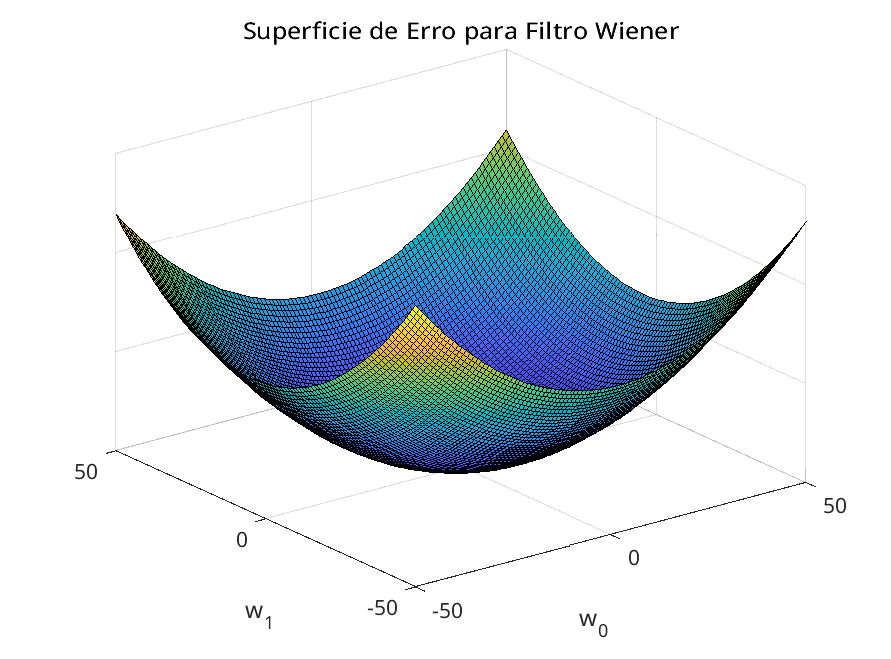
\includegraphics[width=0.5\textwidth]{figs/superficie-de-erro.png}
							\caption{Superfície de erro MSE}
							\label{fig:01}
						\end{figure}
					
				\end{enumerate}
			
		\end{enumerate}
	
	\newpage
	\section*{Algoritmos Recursivos}
	
		\begin{enumerate}
			
			\item Deseja-se minimizar a função objetivo $\mathbb{E}\{e^{4}(n)\}$ utilizando-se um algoritmo do gradiente estocástico do tipo LMS. O algoritmo resultando é chamado de algoritmo least mean fourth (LMF). Derive tal algoritmo. Derive também o filtro ótimo para tal critério e compare as soluções.
			
				\textcolor{red}{Solução:}
				
				Podemos inicialmente definir a função erro para esse filtro como
				
				\begin{align}
					e(n) &= d(n) - y(n), \\
					e(n) &= d(n) - \mathbf{w}^{\text{T}}(n)\mathbf{x}(n),
				\end{align}
				
				e para obtermos a nova expressão de recurssão precisamos primeiro obter o equacionamento para o vetor gradiente instântaneo de $\mathbb{E}\{e^{4}(n)\}$. Isso pode ser prontamente obtido por meio do auxílio de uma derivação implícita

				\begin{align}
					\nabla_{\mathbf{w}} \mathbb{E}\{e^{4}(n)\} &= \frac{\partial \mathbb{E}\{e^{4}(n)\}}{\partial \mathbf{w}} = \mathbb{E}\{ \frac{\partial e^{4}(n)}{\partial \mathbf{w}}\} = \mathbb{E}\{ \frac{\partial e^{4}(n)}{\partial e(n)} \frac{\partial e(n) }{\partial \mathbf{w}}\}, \\
					\nabla_{\mathbf{w}} \mathbb{E}\{e^{4}(n)\} &= \mathbb{E}\{4 e^{3}(n) \frac{\partial (d(n) - \mathbf{w}^{\text{T}}(n)\mathbf{x}(n)) }{\partial \mathbf{w}}\} = \mathbb{E}\{4 e^{3}(n) (0 - \mathbf{x}(n))\}, \\
					\nabla_{\mathbf{w}} \mathbb{E}\{e^{4}(n)\} &= - 4 \mathbb{E}\{e^{3}(n) \mathbf{x}(n)\}.
				\end{align}
			
				Desse modo, para que a minimização de $\mathbb{E}\{e^{4}(n)\}$ seja atingida precisamos garantir apenas que o vetor $x(n)$ tenha entradas ortogonais ao vetor erro $e(n)$. Assim, é necessário que a seguinte equação seja verdade

				\begin{align}
					\mathbb{E}\{e^{3}(n) \mathbf{x}(n)\} &= 0, \\
					\mathbb{E}\{(d(n) - \mathbf{w}^{\text{T}}(n)\mathbf{x}(n))^{3} \mathbf{x}(n)\} &= 0, 
				\end{align}

				onde é possível demonstrar que existe convergência em média para essa expressão se definirmos o passo de aprendizado no seguinte intervalo\footnote{A demonstração da propriedade foi extensivamente explicada no artigo \textit{The Least Mean Square Fourth (LMF) Algorithm and Its Family} de 1984 por Eugene Walash e Bernard Widrow.}

				\begin{align}
					1 < \mu < \frac{1}{6 \sigma^{2}_{z} \lambda_{\text{max}}},
				\end{align}

				onde $\sigma^{2}_{z}$ é a variância do ruído presente e $\lambda_{\text{max}}$ é o maior autovalor da matriz de autocorrelação $\mathbf{R}_{x}$. Por fim, a partir dessas observações podemos escrever a expressão de recurssão para o LMF utilizando 
				a expressão padrão para o algoritmo do gradiente descendente\footnote{Essa expressão é brevemente introduzida no livro texto da disciplina.}

				\begin{align}
					\mathbf{w}(n + 1) &= \mathbf{w}(n) - \mu \mathbf{g}_{w}(n), \\
					\mathbf{w}(n + 1) &= \mathbf{w}(n) + 4 \mu e^{3}(n) \mathbf{x}(n),
				\end{align}

				onde sabemos que o erro é dado por $e(n) = d(n) - \mathbf{w}^{\text{T}}(n)\mathbf{x}(n)$.

			\item Considere o uso de um a sequência de ruído branco com média nula e variância $\sigma^{2}$ como entrada do algoritmo LMS. Avalie
				
				\begin{enumerate}
					
					\item a condição para convergência do algoritmo em média.
					
						\textcolor{red}{Solução:}
						
						A condição de convergência está diretamente associada com o erro nos coeficientes do filtro adaptativo para cada iteração.
						Desse modo, podemos iniciar o estudo desse tópico com a seguinte expressão que relaciona o erro dos coeficientes do filtro de um iteração
						$k$ para a solução ótima
						
						\begin{align}
							\Delta \mathbf{w}(n) = \mathbf{w}(n) - \mathbf{w}_{\text{opt}},
						\end{align}

						e assim podemos reescrever a função de recurssão do LMS do seguinte modo

						\begin{align}
							\Delta \mathbf{w}(n + 1) &= \Delta \mathbf{w}(n) + 2 \mu e(n) \mathbf{x}(n), \\
							\Delta \mathbf{w}(n + 1) &= \Delta \mathbf{w}(n) + 2 \mu \mathbf{x}(n) \left[\mathbf{x}^{\text{T}}(n)\mathbf{w}_{\text{opt}} + z(n) - \mathbf{x}^{\text{T}}(n)\mathbf{w}(n)\right], \\
							\Delta \mathbf{w}(n + 1) &= \Delta \mathbf{w}(n) + 2 \mu \mathbf{x}(n) \left[e_{\text{opt}}(n) - \mathbf{x}^{\text{T}}(n) \Delta \mathbf{w}(n)\right], \\
							\Delta \mathbf{w}(n + 1) &= \left[ \mathbf{I} - 2 \mu \mathbf{x}(n) \mathbf{x}^{\text{T}}(n) \right] \Delta \mathbf{w}(n) + 2 \mu e_{\text{opt}}(n) \mathbf{x}(n)
						\end{align}
					
						onde $z(n) \in \mathcal{N}(0,\sigma^{2})$ e $e_{\text{opt}}(n) = z(n)$. Indicando que, para o caso ideal, teríamos que nos preocupar apenas com o erro introduzido pelas componentes ruidosas do sistema.
						Ademais, também utilizamos o fato de que $e(n) = e^{\text{T}}(n) = \mathbf{w}^{\text{T}}_{\text{opt}}\mathbf{x}(n) + z(n) - \mathbf{w}^{\text{T}}(n)\mathbf{x}(n) = \mathbf{x}^{\text{T}}(n)\mathbf{w}_{\text{opt}} + z(n) - \mathbf{x}^{\text{T}}(n)\mathbf{w}(n)$.
						Em sequência, podemos escrever o valor esperado para o erro como

						\begin{align}
							\mathbb{E}\{\Delta \mathbf{w}(n + 1)\} &= \mathbb{E}\{\left[ \mathbf{I} - 2 \mu \mathbf{x}(n) \mathbf{x}^{\text{T}}(n) \right] \Delta \mathbf{w}(n) + 2 \mu e_{\text{opt}}(n) \mathbf{x}(n)\}, \\
							\mathbb{E}\{\Delta \mathbf{w}(n + 1)\} &= \mathbb{E}\{\left[ \mathbf{I} - 2 \mu \mathbf{x}(n) \mathbf{x}^{\text{T}}(n) \right] \Delta \mathbf{w}(n)\} + 2 \mu \mathbb{E}\{e_{\text{opt}}(n) \mathbf{x}(n)\}
						\end{align}
						
						onde utilizamos a propriedade de linearidade do operador valor esperado. Ao assumirmos que $\mathbf{x}(n)$ é simultaneamente ortogonal aos elementos $e_{\text{opt}}(n)$ e $\Delta \mathbf{w}(n)$ podemos simplificar a expressão acima por
						
						\begin{align}
							\mathbb{E}\{\Delta \mathbf{w}(n + 1)\} &= \left[ \mathbf{I} - 2 \mu \mathbb{E}\{\mathbf{x}(n) \mathbf{x}^{\text{T}}(n)\} \right] \mathbb{E}\{\Delta \mathbf{w}(n)\}, \\
							\mathbb{E}\{\Delta \mathbf{w}(n + 1)\} &= \left( \mathbf{I} - 2 \mu \mathbf{R}_{x} \right) \mathbb{E}\{\Delta \mathbf{w}(n)\},
						\end{align}

						onde podemos utilizar a noção de que $\mathbb{E}\{ \mathbf{I} \} = \mathbf{I}$ uma vez que temos um operador linear. Em continuidade, podemos supor que existe uma matriz $\mathbf{Q}$ unitária que diagonaliza $\mathbf{R}_{x}$
						de tal modo que temos 

						\begin{align}
							\mathbb{E}\{ \mathbf{Q}^{\text{T}} \Delta \mathbf{w}(n + 1) \} &= \left( \mathbf{I} - 2 \mu \mathbf{Q}^{\text{T}} \mathbf{R}_{x} \right) \mathbf{I} \mathbb{E}\{ \Delta \mathbf{w}(n)\}, \\
							\mathbb{E}\{ \mathbf{Q}^{\text{T}} \Delta \mathbf{w}(n + 1) \} &= \left( \mathbf{I} - 2 \mu \mathbf{Q}^{\text{T}} \mathbf{R}_{x} \right) \mathbf{Q} \mathbf{Q}^{\text{T}} \mathbb{E}\{ \Delta \mathbf{w}(n)\}, \\
							\mathbb{E}\{ \mathbf{Q}^{\text{T}} \Delta \mathbf{w}(n + 1) \} &= \left( \mathbf{I} - 2 \mu \mathbf{Q}^{\text{T}} \mathbf{R}_{x} \mathbf{Q} \right) \mathbb{E}\{ \mathbf{Q}^{\text{T}} \Delta \mathbf{w}(n)\}, \\
							\mathbb{E}\{\Delta \mathbf{w}'(n + 1)\} &= \left( \mathbf{I} - 2 \mu \mathbf{\Lambda} \right) \mathbb{E}\{\Delta \mathbf{w}'(n)\}.
						\end{align}

						Podemos, por fim, expandir os termos à esquerda e chegar na seguinte expressão para a análise do comportamento de convergência dos coeficientes de filtro

						\begin{align}
							\mathbb{E}\{ \Delta \mathbf{w}'(n + 1) \} &= \left( \mathbf{I} - 2 \mu \mathbf{\Lambda} \right)^{n + 1} \mathbb{E}\{\Delta \mathbf{w}'(0)\}, \\
							\mathbb{E}\{ \Delta \mathbf{w}'(n + 1) \} &= 
							\begin{bmatrix}
								(1 - 2 \mu \lambda_{1})^{n + 1} & 0 & \cdots & 0 \\
								0 & (1 - 2 \mu \lambda_{2})^{n + 1} & \cdots & \vdots \\
								\vdots & \vdots & \ddots & \vdots \\
								0 & 0 & \cdots & (1 - 2 \mu \lambda_{N})^{n + 1}
							\end{bmatrix} 
							\mathbb{E}\{ \Delta \mathbf{w}'(0)\},	
						\end{align}

						onde temos que $\lambda_{n} \forall n \in \{1, \cdots, N\}$ são os autovalores da matriz de autocorrelação. Portanto, vemos que para garantir a estabilidade da convergência é necessário 
						apenas que o passo de aprendizado do algoritmo seja definido pela seguinte inequação

						\begin{align}
							0 < \mu < \frac{1}{\lambda}_{\text{max}},
						\end{align}

						pois desse modo conseguimos garantir que os valores da diagonal irão tender a zero a medida que o número de iterações do algoritmo tende ao infinito. Ademais, é interessante ressaltar que a escolha 
						do valor de $\mu$ deve também levar em consideração o espalhamento de energia da matriz de correlação. Dessa forma, se não há grande diferença entre
						os valores númericos dos autovalores, então seria aconselhável escolher um passo de aprendizado muito menor do que aquele definido pelo limite superior da expressão obtida acima.
						
						\item o erro em excesso em média quadrática. 
					
						\textcolor{red}{Solução:}
						
						O erro em excesso é normalmente ocasionado pelos termos ruidosos presentes no gradiente, impedindo que os coeficientes convirjam de forma exata para a solução ótima. 
						Podemos iniciar essa análise escrevendo a equação para o erro de estimação para um determinado instante $n$ como se segue

						\begin{align}
							e(n) &= d(n) - \mathbf{w}^{\text{T}}_{\text{opt}} \mathbf{x}(n) - \Delta \mathbf{w}^{\text{T}}(n) \mathbf{x}(n), \\
							e(n) &= e_{\text{opt}}(n) - \Delta \mathbf{w}^{\text{T}}(n) \mathbf{x}(n),
						\end{align}

						onde o erro quadrático é expresso por

						\begin{align}
							e^{2}(n) &= e^{2}_{\text{opt}}(n) - 2 e_{\text{opt}}(n) \Delta \mathbf{w}^{\text{T}}(n) \mathbf{x}(n) + \Delta \mathbf{w}^{\text{T}}(n) \mathbf{x}(n) \mathbf{x}^{\text{T}}(n) \Delta \mathbf{w}(n) ,
						\end{align}

						se definirmos o erro quadrático médio como $\xi(n) = \mathbb{E}\{e^{2}(n)\}$ e o erro ótimo, leia-se mínimo, como $\xi_{\text{min}} = \mathbb{E}\{e^{2}_{\text{opt}}(n)\}$
						então podemos escrever
						
						\begin{align}
							\xi(n) = \xi_{\text{min}} - 2 \mathbb{E}\{e_{\text{opt}}(n) \Delta \mathbf{w}^{\text{T}}(n) \mathbf{x}(n)\} + \mathbb{E}\{\Delta \mathbf{w}^{\text{T}}(n) \mathbf{x}(n) \mathbf{x}^{\text{T}}(n) \Delta \mathbf{w}(n)\},
						\end{align}

						considerando mais uma vez que $\mathbf{x}$ é ortogonal ao $\Delta \mathbf{w}^{\text{T}}(n)$ e ao $e_{\text{opt}}(n)$, simultaneamente, podemos simplificar a expressão ainda mais 

						\begin{align}
							\xi(n) = \xi_{\text{min}} - 2 \mathbb{E}\{\Delta \mathbf{w}^{\text{T}}(n)\} \mathbb{E}\{e_{\text{opt}}(n) \mathbf{x}(n)\} + \mathbb{E}\{\Delta \mathbf{w}^{\text{T}}(n) \mathbf{x}(n) \mathbf{x}^{\text{T}}(n) \Delta \mathbf{w}(n)\},
						\end{align}

						onde podemos utilizar a propriedade $\mathbb{E}\{\Delta \mathbf{w}^{\text{T}}(n) \mathbf{x}(n) \mathbf{x}^{\text{T}}(n) \Delta \mathbf{w}(n)\} = \text{tr}(\mathbb{E}\{\Delta \mathbf{w}^{\text{T}}(n) \mathbf{x}(n) \mathbf{x}^{\text{T}}(n) \Delta \mathbf{w}(n)\})$ uma vez
						que sabemos que o traço de um escalar é o próprio escalar. Sendo assim, utilizando a propriedade cíclica do operador traço escrevemos

						\begin{align}
							\xi(n) &= \xi_{\text{min}} - 2 \mathbb{E}\{\Delta \mathbf{w}^{\text{T}}(n)\} \mathbb{E}\{e_{\text{opt}}(n) \mathbf{x}(n)\} + \text{tr}(\mathbb{E}\{\Delta \mathbf{w}^{\text{T}}(n) \mathbf{x}(n) \mathbf{x}^{\text{T}}(n) \Delta \mathbf{w}(n)\}), \\
							\xi(n) &= \xi_{\text{min}} - 2 \mathbb{E}\{\Delta \mathbf{w}^{\text{T}}(n)\} \mathbb{E}\{e_{\text{opt}}(n)\mathbf{x}(n)\} + \mathbb{E}\{\text{tr}[\Delta \mathbf{w}^{\text{T}}(n) \mathbf{x}(n) \mathbf{x}^{\text{T}}(n) \Delta \mathbf{w}(n)]\}, \\
							\xi(n) &= \xi_{\text{min}} - 2 \mathbb{E}\{\Delta \mathbf{w}^{\text{T}}(n)\} \mathbb{E}\{e_{\text{opt}}(n)\mathbf{x}(n)\} + \mathbb{E}\{\text{tr}[\mathbf{x}(n) \mathbf{x}^{\text{T}}(n) \Delta \mathbf{w}(n) \Delta \mathbf{w}^{\text{T}}(n)]\}, \\
							\xi(n) &= \xi_{\text{min}} + \mathbb{E}\{\text{tr}[\mathbf{x}(n) \mathbf{x}^{\text{T}}(n) \Delta \mathbf{w}(n) \Delta \mathbf{w}^{\text{T}}(n)]\}, \\
							\xi(n) &= \xi_{\text{min}} + \text{tr}(\mathbb{E}\{\mathbf{x}(n) \mathbf{x}^{\text{T}}(n) \Delta \mathbf{w}(n) \Delta \mathbf{w}^{\text{T}}(n)\}), \\
							\xi(n) &= \xi_{\text{min}} + \text{tr}(\mathbb{E}\{\mathbf{x}(n) \mathbf{x}^{\text{T}}(n)\} \mathbb{E}\{\Delta \mathbf{w}(n) \Delta \mathbf{w}^{\text{T}}(n)\}), \\
							\xi(n) &= \xi_{\text{min}} + \text{tr}(\mathbf{R}_{x} \mathbb{E}\{\Delta \mathbf{w}(n) \Delta \mathbf{w}^{\text{T}}(n)\}), \\
							\xi(n) &= \xi_{\text{min}} + \text{tr}(\mathbb{E}\{\mathbf{R}_{x} \Delta \mathbf{w}(n) \Delta \mathbf{w}^{\text{T}}(n)\}), 
						\end{align}

						onde o processo justifica-se pela intercambialidade entre os operadores traço e valor esperador e pela ortogonalidade mencionada anteriormente. Em sequência podemos definir o erro em excesso por

						\begin{align}
							\xi(n) - \xi_{\text{min}} &= \text{tr}(\mathbb{E}\{\mathbf{R}_{x} \Delta \mathbf{w}(n) \Delta \mathbf{w}^{\text{T}}(n)\}), \\
							\Delta \xi(n) &= \text{tr}(\mathbb{E}\{\mathbf{R}_{x} \Delta \mathbf{w}(n) \Delta \mathbf{w}^{\text{T}}(n)\}), \label{excesso1}
						\end{align}

						e adicionalmente, pela definição de uma transformação de similaridade onde garantimos que exista $\mathbf{Q} \mathbf{Q}^{\text{T}} = \mathbf{I}$ capaz de diagonalizar a matriz de autocorrelação, podemos reescrever a Equação (\ref{excesso1}) da seguinte forma

						\begin{align}
							\Delta \xi(n) &= \text{tr}(\mathbb{E}\{\mathbf{Q} \mathbf{Q}^{\text{T}} \mathbf{R}_{x} \mathbf{Q} \mathbf{Q}^{\text{T}} \Delta \mathbf{w}(n) \Delta \mathbf{w}^{\text{T}}(n) \mathbf{Q} \mathbf{Q}^{\text{T}}\}), \\
							\Delta \xi(n) &= \text{tr}(\mathbb{E}\{\mathbf{Q} \mathbf{\Lambda} \mathbf{Q}^{\text{T}} \Delta \mathbf{w}(n) \Delta \mathbf{w}^{\text{T}}(n) \mathbf{Q} \mathbf{Q}^{\text{T}}\}), \\
							\Delta \xi(n) &= \text{tr}(\mathbb{E}\{\mathbf{Q} \mathbf{\Lambda} \text{cov} \left[\Delta \mathbf{w}'(n)\right] \mathbf{Q}^{\text{T}}\}), \\
							\Delta \xi(n) &= \text{tr}(\mathbb{E}\{\mathbf{\Lambda} \text{cov} \left[\Delta \mathbf{w}'(n)\right] \mathbf{Q}^{\text{T}} \mathbf{Q}\}), \\
							\Delta \xi(n) &= \text{tr}(\mathbb{E}\{\mathbf{\Lambda} \text{cov} \left[\Delta \mathbf{w}'(n)\right]\}), \label{excesso2}
						\end{align}

						onde é sabido que $\text{cov} \left[\Delta \mathbf{w}(n)\right] = \mathbb{E}\{(\mathbf{w}(n) - \mathbf{w}_{\text{opt}}) (\mathbf{w}(n) - \mathbf{w}_{\text{opt}})^{\text{T}}\}$ e $\Delta \mathbf{w}'(n) = \mathbf{Q}^{\text{T}} \Delta \mathbf{w}(n) \Delta \mathbf{w}^{\text{T}}(n) \mathbf{Q}$.
						Enfim, a partir das orientações presentes no livro texto da disciplina a respeito da matriz de covariância do vetor de erros é possível ainda escrever a Equação (\ref{excesso2}) como

						\begin{align}
							\Delta \xi(n) &= \sum^{N}_{i = 1} \lambda_{i} v_{i}'(n) = \mathbf{\lambda}^{\text{T}} \mathbf{v}'(n),
						\end{align}

						onde $\mathbf{\lambda}$ é um vetor contendo todos os autovalores da matriz de autocorrelação e $\mathbf{v}(n)$ é um vetor que contém os elementos da diagonal de $\text{cov} \left[\Delta \mathbf{w}'(n)\right]$. Em suma, podemos 
						expressar o $i$th elemento do vetor diagonal $\mathbf{v}'(n + 1)$, seguindo orientações disponíveis no livro texto da disciplina, com o seguinte equacionamento

						\begin{align}
							v_{i}'(n + 1) &= (1 - 4 \mu \lambda_{i} + 8 \mu^{2} \lambda^{2}_{i}) v_{i}'(n) + 4 \mu^{2} \lambda_{i} \sum^{N}_{j = 0} \lambda_{j} v_{j}'(n) + 4 \mu^{2} \sigma^{2}_{z} \lambda_{i}.
						\end{align}

						Entretanto, se considerarmos que $v_{i}'(n + 1) \approx v_{i}'(n)$ quando $n \rightarrow \infty$ podemos simplificar a expressão, além de que 
						também podemos realizar uma operação de soma total dos parâmetros para obter o erro em excesso total

						\begin{align}
							\notag &\sum^{N}_{i = 1} v_{i}'(n) = \sum^{N}_{i = 1} (1 - 4 \mu \lambda_{i} + 8 \mu^{2} \lambda^{2}_{i}) v_{i}'(n) + 4 \mu^{2} \sum^{N}_{i = 1} \lambda_{i} \sum^{N}_{j = 0} \lambda_{j} v_{j}'(n) + 4 \mu^{2} \sigma^{2}_{z} \sum^{N}_{i = 1} \lambda_{i}, \\
							\notag &\sum^{N}_{i = 1} v_{i}'(n) = \sum^{N}_{i = 1} v_{i}'(n) - 4 \mu \sum^{N}_{i = 1} \lambda_{i} v_{i}'(n)  + 8 \mu^{2} \sum^{N}_{i = 1} \lambda^{2}_{i} v_{i}'(n) + 4 \mu^{2} \sum^{N}_{i = 1} \lambda_{i} \sum^{N}_{j = 0} \lambda_{j} v_{j}'(n) + 4 \mu^{2} \sigma^{2}_{z} \sum^{N}_{i = 1} \lambda_{i}, \\
							\notag &\sum^{N}_{i = 1} v_{i}'(n) - \sum^{N}_{i = 1} v_{i}'(n) + 4 \mu \sum^{N}_{i = 1} \lambda_{i} v_{i}'(n) - 4 \mu^{2} \sum^{N}_{i = 1} \lambda_{i} \sum^{N}_{j = 0} \lambda_{j} v_{j}'(n) = 4 \mu^{2} \sigma^{2}_{z} \sum^{N}_{i = 1} \lambda_{i} + 8 \mu^{2} \sum^{N}_{i = 1} \lambda^{2}_{i} v_{i}'(n), \\
							\notag &4 \mu \sum^{N}_{j = 1} \lambda_{j} v_{j}'(n)(1 - \mu \sum^{N}_{i = 1} \lambda_{i}) = 4 \mu (\mu \sigma^{2}_{z} \sum^{N}_{i = 1} \lambda_{i} + 2 \mu \sum^{N}_{i = 1} \lambda^{2}_{i} v_{i}'(n)), \\
							\notag &\sum^{N}_{j = 1} \lambda_{j} v_{j}'(n) = \frac{\mu \sigma^{2}_{z} \sum^{N}_{i = 1} \lambda_{i} + 2 \mu \sum^{N}_{i = 1} \lambda^{2}_{i} v_{i}'(n)}{1 - \mu \sum^{N}_{i = 1} \lambda_{i}}, \\
							\notag &\sum^{N}_{j = 1} \lambda_{j} v_{j}'(n) \approx \frac{\mu \sigma^{2}_{z} \sum^{N}_{i = 1} \lambda_{i} }{1 - \mu \sum^{N}_{i = 1} \lambda_{i}}, \\
							&\sum^{N}_{j = 1} \lambda_{j} v_{j}'(n) = \frac{\mu \sigma^{2}_{z} \text{tr}(\mathbf{R}_{x})}{1 - \mu \text{tr}(\mathbf{R}_{x})},
						\end{align}

						onde foi considerado que o termo $2 \mu \sum^{N}_{i = 1} \lambda^{2}_{i} v_{i}'(n)$ apresenta contribuição insignificante para o valor absoluto do numerador. Entretanto, é mencionado no livro texto que tal aproximação é de prova complexa, mas que normalmente 
						se verifica verdadeira para pequenos valores do passo de aprendizado $\mu$. Portanto, o erro em excesso pode ser prontamente descrito pela expressão que se segue

						\begin{align}
							\xi_{\text{excesso}} &= \underset{n \rightarrow \infty}{\text{lim}} \Delta \xi(n) \approx \frac{\mu \sigma^{2}_{z} \text{tr}(\mathbf{R}_{x})}{1 - \mu \text{tr}(\mathbf{R}_{x})}.
						\end{align}

						Vale ainda expor que podemos considerar $1 - \mu \text{tr}(\mathbf{R}_{x}) \approx 1$ para valores muito pequenos de $\mu$, obtendo assim uma versão aproximada para o erro em excesso dada por
						
						\begin{align}
							\xi_{\text{excesso}} &= \underset{n \rightarrow \infty}{\text{lim}} \Delta \xi(n) \approx \mu \sigma^{2}_{z} \text{tr}(\mathbf{R}_{x}).
						\end{align}

				\end{enumerate}

			\item Avalie a questão anterior para o caso do algoritmo LMS-Normalizado. Compare os dois casos.
				
			\textcolor{red}{Solução:}

			Em acordância com o livro texto da disciplina a expressão de atualização dos coeficientes de filtro para o algoritmo NLMS é dada por

			\begin{align}
				\mathbf{w}(k+1) = \mathbf{w}(k) + \frac{\mu_{norm}}{\gamma + \mathbf{x}^{\text{T}}(k) \mathbf{x}(k)} \mathbf{e}(k) \mathbf{x}(k),
			\end{align}

			e considerando que o valor médio do passo de aprendizado aplicado na direção LMS $2 \mathbf{e}(k) \mathbf{x}(k)$ é descrito por $\frac{\mu_{norm}}{2 \text{tr}(\mathbf{R_{xx}})}$, então é possível chegar
			no seguinte limite superior para o valor de convergência se compararmos diretamente as fórmulas de atualização do LMS padrão com o LMS normalizado

			\begin{align}
				0 &< \frac{\mu_{norm}}{2 \text{tr}(\mathbf{R_{xx}})} < \frac{1}{\text{tr}(\mathbf{R_{xx}})}, \\
				0 &< \mu_{norm} < 2, 
			\end{align}
						
			\item Considere um sinal branco gaussiano de variância unitária transmitido por um canal de comunicação de função de transferência $H(z) = 1 + 1.6z^{-1}$. Para compensar este
			canal utiliza-se um equalizador dado por $W(z) = w_{0} + w_{1}z^{-1}$ .
			
			
				\begin{enumerate}
					
					\item Forneça o equalizador ótimo segundo o critério de Wiener. Esboce a posição dos zeros do canal e do equalizador no plano Z.
					
						\textcolor{red}{Solução:}
						
						Considerando um sinal gaussiano branco $x(n)$ a saída do canal pode ser prontamente obtida por
						
						\begin{align}
							y(n) = x(n) + 1.6 x(n - 1),
						\end{align}
						
						e a matriz de autocorrelação será então dada por
						
						\begin{align}
							\mathbf{R}_{y} =
							\begin{bmatrix}
								\mathbb{E}\{y(n)y^{\text{H}}(n)\} & \mathbb{E}\{y(n)y^{\text{H}}(n - 1)\} \\
								\mathbb{E}\{y(n - 1)y^{\text{H}}(n)\} & \mathbb{E}\{y(n - 1)y^{\text{H}}(n - 1)\}
							\end{bmatrix},
						\end{align}
						
						onde podemos calcular os valores teóricos para as correlações da seguinte forma se assumirmos que existe independência entre amostras distintas e que o sinal é média nula 
						
						\begin{align*}
							\mathbb{E}\{y(n)y^{\text{H}}(n)\} &= \mathbb{E}\{ \mathbf{x}^{2}(n) + 1.6 \mathbf{x}(n) \mathbf{x}^{\text{H}}(n - 1) + 1.6 \mathbf{x}(n - 1) \mathbf{x}^{\text{H}} (n) \\
							&+ 2.56 \mathbf{x}^{2}(n - 1) \} = 3.56, \\
							\mathbb{E}\{y(n)y^{\text{H}}(n - 1)\} &= \mathbb{E}\{ \mathbf{x}(n) \mathbf{x}^{\text{H}}(n - 1) + 1.6 \mathbf{x}(n) \mathbf{x}^{\text{H}}(n - 2) + 1.6 \mathbf{x}(n - 1) \mathbf{x}^{\text{H}} (n - 1) \\ 
							&+ 2.56 \mathbf{x}(n - 1) \mathbf{x}^{\text{H}}(n - 2) \} = 1.60, \\
							\mathbb{E}\{y(n - 1)y^{\text{H}}(n)\} &= \mathbb{E}\{ \mathbf{x}(n - 1) \mathbf{x}^{\text{H}}(n) + 1.6 \mathbf{x}(n - 1) \mathbf{x}^{\text{H}}(n - 1) + 1.6 \mathbf{x}(n - 2) \mathbf{x}^{\text{H}} (n) \\ 
							&+ 2.56 \mathbf{x}(n - 2) \mathbf{x}^{\text{H}}(n - 1) \} = 1.60, \\
							\mathbb{E}\{y(n - 1)y^{\text{H}}(n - 1)\} &= \mathbb{E}\{ \mathbf{x}^{2}(n - 1) + 1.6 \mathbf{x}(n - 1) \mathbf{x}^{\text{H}}(n - 2) + 1.6 \mathbf{x}(n - 2) \mathbf{x}^{\text{H}} (n - 1) \\ 
							&+ 2.56 \mathbf{x}(n - 2)^{2} \} = 3.56, \\
						\end{align*}
						
						podendo assim descrever a matriz de autocorrelação teórica e sua inversa como
						
						\begin{align}
							\mathbf{R}_{y} =
							\begin{bmatrix}
								3.56 & 1.60 \\
								1.60 & 3.56
							\end{bmatrix},
						\end{align}
						
						\begin{align}
							\mathbf{R}^{-1}_{y} = \frac{1}{3.56^{2} - 1.6^{2}}
							\begin{bmatrix}
								3.56 &  -1.60 \\
								-1.60 & 3.56
							\end{bmatrix} =
							\begin{bmatrix}
								0.35 &  -0.16 \\
								-0.16 & 0.35
							\end{bmatrix}.
						\end{align}
						
						Já o vetor de correlação cruzada teórico pode ser descrito por
						
						\begin{align}
							\mathbf{p}_{yd} =
							\begin{bmatrix}
								\mathbb{E}\{y(n)d(n)\} \\
								\mathbb{E}\{y(n - 1)d(n)\}
							\end{bmatrix} = 
							\begin{bmatrix}
								1 \\
								0
							\end{bmatrix},
						\end{align}
						
						pois queremos que o sinal de saída tenha a maior correlação possivel com o sinal desejado de um mesmo instante mas continue sendo independente de um sinal de um instante temporal diferente.
						Desse modo, podemos obter o equalizador ótimo segundo o critério de Wiener como
						
						\begin{align}
							\mathbf{w}_{\text{opt}} = \mathbf{R}^{-1}_{y} \mathbf{p}_{yd} = \begin{bmatrix}
								0.35 \\
								-0.16
							\end{bmatrix}.
						\end{align}
						
						Por fim, abaixo segue o traçado para os zeros das funções de transferência tanto do canal quanto do filtro ótimo em azul e em vermelho, respectivamente.
						
						\begin{figure}[!ht]
							\centering
							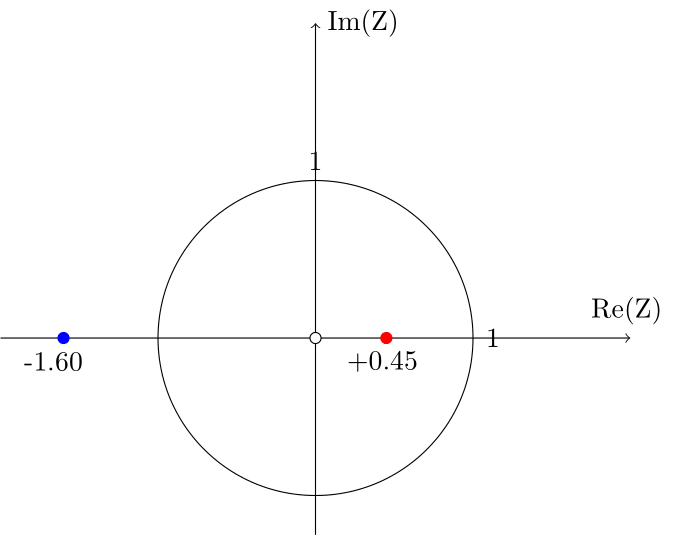
\includegraphics[width=0.5\textwidth]{figs/plano_z.png}
							\caption{Zeros do canal e do equalizador no plano-z.}
						\end{figure}
					
					\item Obtenha o filtro de erro de predição direta de passo unitário, correspondente ao sinal à saída do canal. Calcule os zeros deste filtro e compare com os do equalizador.
					
						\textcolor{red}{Solução:}

						De forma semelhante ao abordado anteriormente temos que o filtro de predição direta de passo unitário é dado por
						
						\begin{align}
							\hat{x}(n) &= \sum^{M + k - 1}_{i = k} w_{f,i} x(n - i) = \sum^{2}_{i = 1} w_{f,i} x(n - i) = \mathbf{w}^{\text{T}}_{f} \mathbf{x}(n - 1),
						\end{align}

						onde o erro quadrático médio é dado por

						\begin{align}
							\mathbb{E}\{e^{2}(n)\} = \mathbb{E}\{(x(n) - \hat{x}(n) )^{2}\} = \mathbf{r}_{x}(0) - 2 \mathbf{w}^{\text{T}}_{f} \mathbf{r}_{x,f} + \mathbf{w}^{\text{T}}_{f} \mathbf{R}_{x} \mathbf{w}_{f},
						\end{align}

						onde a solução ótima será dada por

						\begin{align}
							\mathbf{w}_{f,\text{opt}} = \mathbf{R}^{-1}_{x} \mathbf{r}_{x,f}.
						\end{align}

						Onde teremos que a mesma matriz de autocorrelação e o vetor de correlação cruzada serão definidos por

						\begin{align}
							\mathbf{R}_{y} &=
							\begin{bmatrix}
								3.56 & 1.60 \\
								1.60 & 3.56
							\end{bmatrix}, \\
							\mathbf{r}_{y,f} &= 
							\begin{bmatrix}
								r_{y}(1) \\
								r_{y}(2)
							\end{bmatrix} =
							\begin{bmatrix}
								\mathbb{E}\{y(n) y(n - 1)\} \\
								\mathbb{E}\{y(n) y(n - 2)\}
							\end{bmatrix} = 
							\begin{bmatrix}
								1.60 \\
								0
							\end{bmatrix}.
						\end{align}

						Por essa razão temos

						\begin{align}
							\mathbf{w}_{f,\text{opt}} = 
							\begin{bmatrix}
								0.35 & -0.16 \\
								-0.16 & 0.35
							\end{bmatrix}
							\begin{bmatrix}
								1.60 \\
								0
							\end{bmatrix} =
							\begin{bmatrix}
								0.56 \\
								-0.26
							\end{bmatrix}.
						\end{align}

						Em seguida, podemos obter os zeros do filtro como

						\begin{align}
							W(z) &= 0.56 - 0.26 z^{-1}, \\
							0 &= 0.56 - 0.26 z^{-1}, \\
							z &= 0.45,
						\end{align}

						que é o mesmo zero do equalizador definido anteriormente.

					\newpage
					\item Obtenha as trajetórias sobre as curvas de nível, tendo condições iniciais nulas para os coeficientes do equalizador, para os seguintes algoritmos: (a) Algoritmo de Newton, (b) Gradiente Determinístico, (c) Least Means Square e (d) Least Means Square Normalizado
						
						\textcolor{red}{Solução:}
						
						Antes de tudo é necessário definir a superfície de erro que servirá como referência para traçar as curvas de nível. Desse modo, podemos prontamente
						definir a superfície MSE como
						
						\begin{align}
							\mathbf{J}(w) &= \mathbb{E}\{e^{2}(n)\}, \\
							\mathbf{J}(w) &= \sigma^{2}_{d} - 2\mathbf{w}^{T}\mathbf{p}_{xd} + w^{T}\mathbf{R}_{X}\mathbf{w}. \label{mseopt}  
						\end{align}
						
						Desse modo, nas Figuras \ref{fig:newton_contour}, \ref{fig:gradient_contour}, \ref{fig:lms_contour} e \ref{fig:nlms_contour} temos as curvas de convergência do algoritmo sobre a superficie MSE descrita na Equação (\ref{mseopt}). 

					\item Obtenha também a evolução do erro quadrático médio para cada um dos algoritmos anteriores.
						
						\textcolor{red}{Solução:}

						A evolução do erro quadrático médio está disponível nas Figuras \ref{fig:newton_mse}, \ref{fig:gradient_mse}, \ref{fig:lms_mse} e \ref{fig:nlms_mse} para cada um dos algoritmos requeridos.
					
					\item Qual o número de condicionamento para o problema em questão?
					
						\textcolor{red}{Solução:}
						
						o número de condicionamento pode ser prontamente obtido pela expressão

						\begin{align}
							\mathbb{C} (\mathbf{R}_{x}) = \frac{\lambda_{\text{max}}}{\lambda_{\text{min}}},
						\end{align}
					
						onde $\lambda_{\text{max}}$ e $\lambda_{\text{min}}$ são os autovalores máximo e mínimo da matriz de autocorrelação, respectivamente. Por meio de um software
						matemático foi possível obter os seguinte autovalores para a matriz de autocorrelação teórica

						\begin{align}
							\mathbb{C} (\mathbf{R}_{x}) = \frac{5.16}{1.96} = 2.63,
						\end{align}

						onde talvez seja importante ressaltar que também poderiamos ter obtido os autovalores resolvendo a equação do polinômio
						característico da matriz de autocorrelação que é dada por

						\begin{align}
							\lambda^{2} - 7.12 \lambda + 10.11 = 0. 
						\end{align}

					\item Qual deveria ser o canal para que o número de condicionamento fosse menor/maior que 5?
					Comente os resultados.
					
						\textcolor{red}{Solução:}
						
						Inicialmente podemos escrever a matriz de correlação contabilizando a contribuição dos coeficientes do canal para os elementos individuais
						
						\begin{align}
							\mathbf{R}_{y} =
							\begin{bmatrix}
								a_{0} + a^{2}_{1} & a_{1}\\
								a_{1} & a_{0} + a^{2}_{1}
							\end{bmatrix},
						\end{align}

						onde a função de transferência do canal seria dada por $H(z) = a_{0} + a_{1}z^{-1}$. A partir dessa matriz de autocorrelação genérica podemos então 
						definir o seguinte polinômio característico

						\begin{align}
							&(\lambda - a_{0} + a^{2}_{1})^{2} - a^{2}_{1} = 0, \\
							&\lambda^{2} \underbrace{- 2 (a_{0} + a^{2}_{1})}_{b} \lambda + \underbrace{(a_{0} + a^{2}_{1})^{2} - a^{2}_{1}}_{c} = 0, \\
							&\lambda^{2} + b \lambda + c = 0,
						\end{align}

						onde sabemos que a solução é facilmente obtida pela fórmula de Bháskara. A partir disso podemos definir o número de condicionamento como

						\begin{align}
							\mathbb{C} (\mathbf{R}_{x}) &= \frac{\lambda_{\text{max}}}{\lambda_{\text{min}}}, \\
							\mathbb{C} (\mathbf{R}_{x}) &= \frac{- b + \sqrt{b^{2} - 4c}}{- b - \sqrt{b^{2} - 4c}}, \\
							\mathbb{C} (\mathbf{R}_{x}) &= \frac{2 (a_{0} + a^{2}_{1}) + \sqrt{4 (a_{0} + a^{2}_{1})^{2} - 4 (a_{0} + a^{2}_{1})^{2} + 4 a^{2}_{1}}}{2 (a_{0} + a^{2}_{1}) - \sqrt{4 (a_{0} + a^{2}_{1})^{2} - 4 (a_{0} + a^{2}_{1})^{2} + 4 a^{2}_{1}}}, \\
							\mathbb{C} (\mathbf{R}_{x}) &= \frac{2 (a_{0} + a^{2}_{1}) + 2a_{1}}{2 (a_{0} + a^{2}_{1}) - 2a_{1}}, \\
							\mathbb{C} (\mathbf{R}_{x}) &= \frac{a_{0} + a^{2}_{1} + a_{1}}{a_{0} + a^{2}_{1} - a_{1}},
						\end{align}

						assim temos agora uma fórmula para o número de condicionamento da matriz de autocorrelação com base nos coeficientes de canal. A partir disso basta que as seguintes inequações sejam atendidas para que
						obtenhamos um número de condicionamento maior ou menor do que o requerido

						\begin{align}
							a_{0} + a^{2}_{1} + a_{1} &\geq 5 (a_{0} + a^{2}_{1} - a_{1}), \\
							a_{0} + a^{2}_{1} + a_{1} &\leq 5 (a_{0} + a^{2}_{1} - a_{1}).
						\end{align}

				\end{enumerate}
			
			\item Utilize o algoritmo LMS para identificar um sistema com a função de transferência dada abaixo.
			
				\begin{align}
					H(z) = \frac{1 - z^{-12}}{1 - z^{-1}}
				\end{align}
			
				\begin{enumerate}
					
					\item Calcule o limite superior para $\mu$ (ou seja $\mu_{\text{max}}$) para garantir a estabilidade do algoritmo.
					
						\textcolor{red}{Solução:}
					
						Para garantirmos a estabilidade do algoritmo precisamos apenas obter o valor numérico do maior autovalor definido pela matriz de autocorrelação do problema.
						Desse modo, podemos simplificar a função de transferência por meio da seguinte manipulação algébrica

						\begin{align*}
							H(z) &= \frac{1 - z^{-12}}{1 - z^{-1}}, \\
							H(z) &= \frac{(1 - z^{-1})(1 + z^{-1} + z^{-2} + z^{-3} + z^{-4} + z^{-5} + z^{-6} + z^{-7} + z^{-8} + z^{-9} + z^{-10} + z^{-11})}{1 - z^{-1}}, \\
							H(z) &= 1 + z^{-1} + z^{-2} + z^{-3} + z^{-4} + z^{-5} + z^{-6} + z^{-7} + z^{-8} + z^{-9} + z^{-10} + z^{-11},
						\end{align*}

						e tomando a transformada z inversa da função de transferência chega-se a seguinte saída de um sinal transmitido por esse canal

						\begin{align*}
							y(n) &= x(n) + x(n-1) + x(n-2) + x(n-3) + x(n-4) + x(n-5) + x(n-6) + x(n-7) \\
							&+ x(n-8) + x(n-9) + x(n-10) - x(n-11), 
						\end{align*}

						Em sequência é possível utilizar um software matemático para a realizar a obtenção da matriz de autocorrelação estimada

						\begin{figure}[ht!]
							\centering
							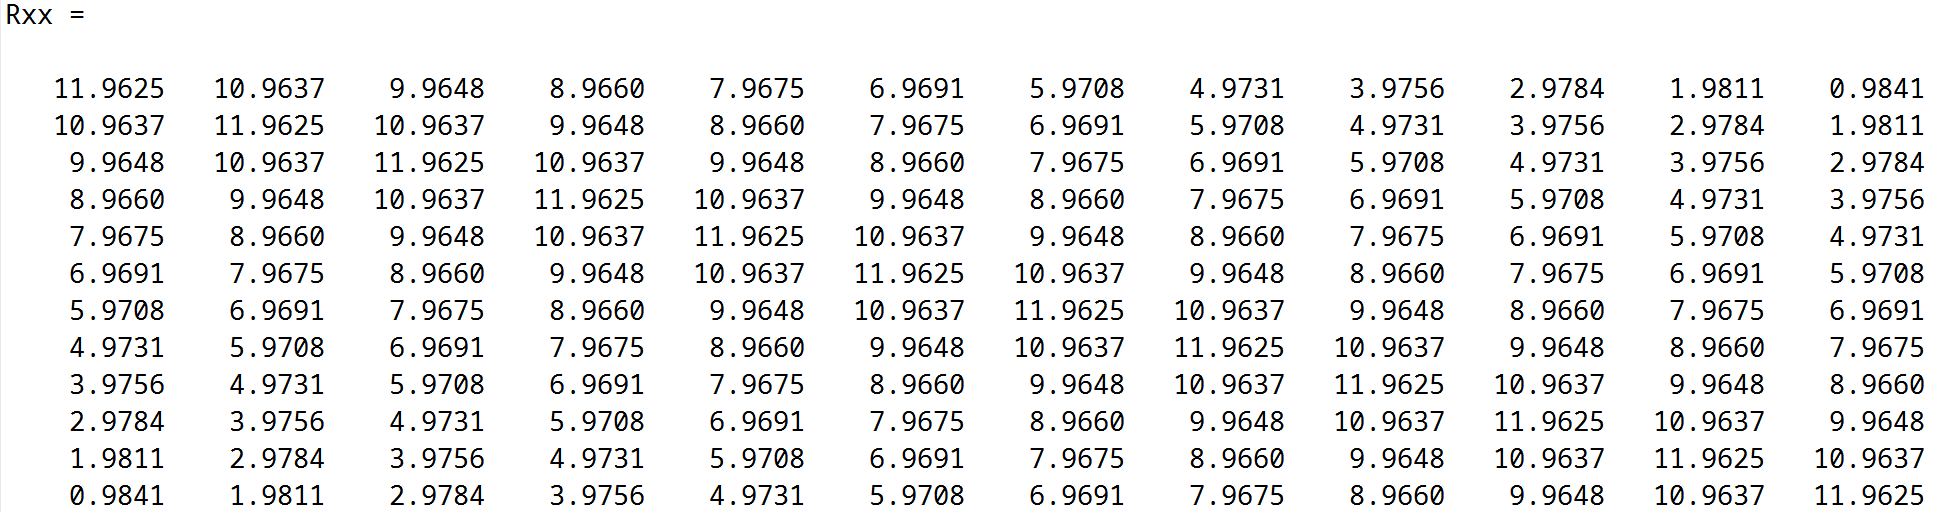
\includegraphics[width=1\textwidth]{figs/Rxx.png}
						\caption{Matriz de autocorrelação estimada após 10000 realizações para retirada do comportamento médio}
						\label{fig:rxx}
						\end{figure}

						onde a análise de autovalores de $\mathbf{R}_{xx}$ resulta no seguinte intervalo de convergência para o passo de 
						aprendizado

						\begin{align}
							0 < \mu < \frac{1}{\lambda_{\text{max}}} = \frac{1}{195} \approx 0.005,
						\end{align}

						e assim $\mu_{\text{max}} \approx 0.005$.

					\item Execute o algoritmo para $\frac{\mu_{\text{max}}}{2}$, $\frac{\mu_{\text{max}}}{10}$ e $\frac{\mu_{\text{max}}}{50}$. Comente sobre o comportamento da convergência de cada caso.
						
						\textcolor{red}{Solução:}

						Nas Figuras \ref{fig:mu_2}, \ref{fig:mu_10} e \ref{fig:mu_50} podemos verificar a convergência do algoritmo para esse problema. 

					\item Meça o desajuste (misadjustment) em cada exemplo e comparar com os resultados obtidos pela solução teórica (Eq. (3.50) do livro texto)					

						\textcolor{red}{Solução:}

						O desajuste pode ser aproximado por

						\begin{align}
							M = \frac{\xi_{\text{excesso}}}{\xi_{\text{min}}} &\approx \frac{\mu \text{tr}(\mathbf{R}_{x})}{1 - \mu \text{tr}(\mathbf{R}_{x})},
						\end{align}

						e a partir dessa expressão foi possivel obter a seguinte tabela

						\begin{table}[!ht]
							\centering
							\begin{tabular}{|l|l|l|}
								\hline
							 	& Empírico & Téorico \\ \hline
							 	$\frac{\mu_{\text{max}}}{2}$ & $ -1.1618 $ &  $ -1.1613 $ \\ \hline
							 	$\frac{\mu_{\text{max}}}{10}$ & $ -3.2938 $ & $ -3.2727 $ \\ \hline
							 	$\frac{\mu_{\text{max}}}{50}$ & $ +0.4029 $ & $ +0.4045 $ \\ \hline
							\end{tabular}
						\end{table}

						Os resultados foram obtidos por uso de software matemático e os códigos estão disponíveis juntamente com este relatório.

					\item Mostre o gráfico da resposta em frequência do filtro FIR em qualquer uma das iterações após a convergência ser obtida e compare com o sistema desconhecido.
					
						\textcolor{red}{Solução:}

						A resposta em frequência do filtro está disponível na Figura \ref{fig:filter_response}. 

				\end{enumerate}
			
			\item Seja o canal de comunicações dado por
			
				\begin{align}
					H(z) = 0.5 + 1.2z^{-1} + 1.5z^{-2} + z^{-3},
				\end{align}
				
				e deseja-se projetar um equalizar para o mesmo. A estrutura do equalizador é mostrada na Figura abaixo. Os símbolos $s(n)$ são transmitidos através de um canal e corrompidos por ruído aditivo gaussiano branco complexo $v(n)$. O sinal recebido $x(n)$ é processado pelo equalizador FIR para gerar estimativas $\overset{\sim}{s}(n - \delta)$, as quais são passados por um dispositivo decisor gerando  símbolos $\hat{s}(n - \delta)$. O equalizador possui dois modos de operação: um modo de treinamento durante o qual uma versão atrasada e  replicada da sequência de entrada é usada como o sinal de referência (desejado) e um modo dirigido por decisão no qual a saída do dispositivo de decisão substitui a sequência de referência. O sinal de entrada $s(n)$ é escolhido de uma constelação QAM (por exemplo, 4-QAM, 16-QAM, 64-QAM ou 256-QAM).
				
				\begin{figure}[!ht]
					\centering
					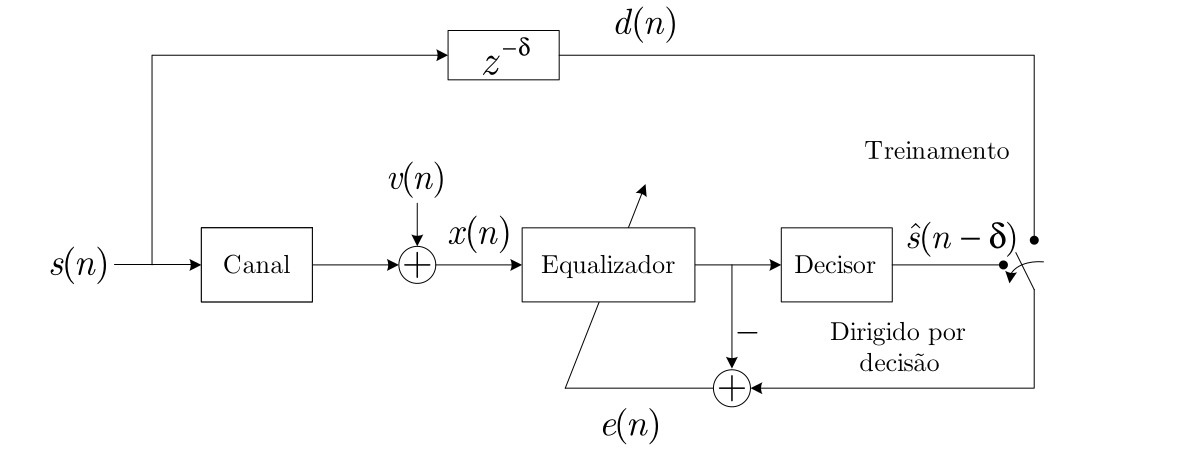
\includegraphics[width=0.85\textwidth]{figs/equalizador_linear.png}
					\caption{Equalizador Linear}
				\end{figure}
			
				\begin{enumerate}
					
					\item Faça um programa que treine o filtro adaptativo com 500 símbolos de uma constelação 4-QAM, seguindo de uma operação dirigida por decisão de 5000 símbolos de uma constelação 16-QAM. Escolha a variância do ruído $\sigma^{2}_{v}$ de maneira que ela promova uma relação sinal ruído de 30 db na entrada do equalizador. Note que os símbolos escolhidos não têm variância unitária. Por esta razão, a a variância do ruído necessita ser ajustada adequadamente para cada uma das diferentes modulações (constelações) QAM para fornecer o nível de SNR desejado. Escolha $\delta = 15$ e o comprimento do equalizador M = 15. Mostre os gráficos da evolução temporal de $s(n)$, $x(n)$ e $\overset{\sim}{s}(n - \delta)$. Use o LMS-normalizado com um fator de passo de $\mu = 0.4$.
								
						\textcolor{red}{Solução:}

						Os resultados estão nas Figuras \ref{fig:L3Q6A1} e \ref{fig:L3Q6A2}.

					\item Para os mesmos parâmetros do item (a), plote e compare os gráficos de evolução que seriam resultante se o equalizador fosse treinado com 150, 300 e 500 iterações. Use o LMS com um
					$\mu = 0.001$.
					
						\textcolor{red}{Solução:}

						Os resultados estão na Figura \ref{fig:L3Q6B}.

					\item Assuma agora que os dados transmitidos foram gerados de uma constelação 256-QAM ao invés de 16-QAM. Plote os gráficos da evolução do sinal na saída do equalizador quando treinado
					usando o LMS-normalizado e 500 símbolos de treinamento.					
					
						\textcolor{red}{Solução:}

						Os resultados estão nas Figuras \ref{fig:L3Q6C1} e \ref{fig:L3Q6C2}.

					\item Gerar as curvas de taxa de erro de símbolo (SER, do inglês Symbol Error Rate) versus SNR na entrada do equalizador para símbolos de constelações 4, 16, 64 e 256-QAM. Faça SNR variar
					de 5dB a 30dB.
					
						\textcolor{red}{Solução:}

						Os resultados estão na Figura \ref{fig:L3Q6D}.

				\end{enumerate}
				
				\newpage
				\begin{figure}[!ht]
					\centering
					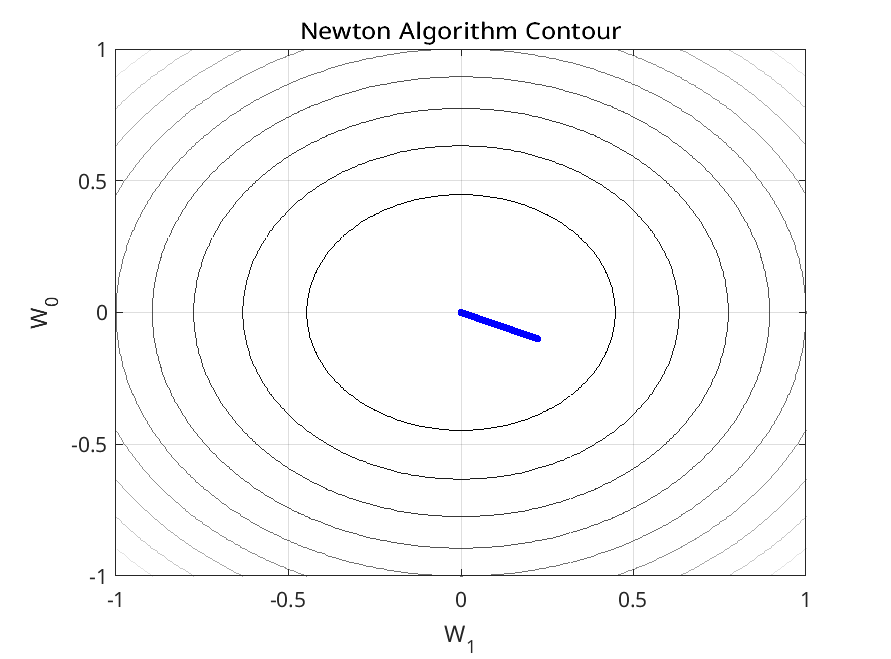
\includegraphics[width=0.75\textwidth]{figs/newton_contour.png}
					\caption{Caminho de convergência na superficie MSE para o Método de Newton. $\text{Amostras} = 5000$, $M = 2$, $\mu = 10^{-3}$}
					\label{fig:newton_contour}
				\end{figure}
				
				\begin{figure}[!ht]
					\centering
					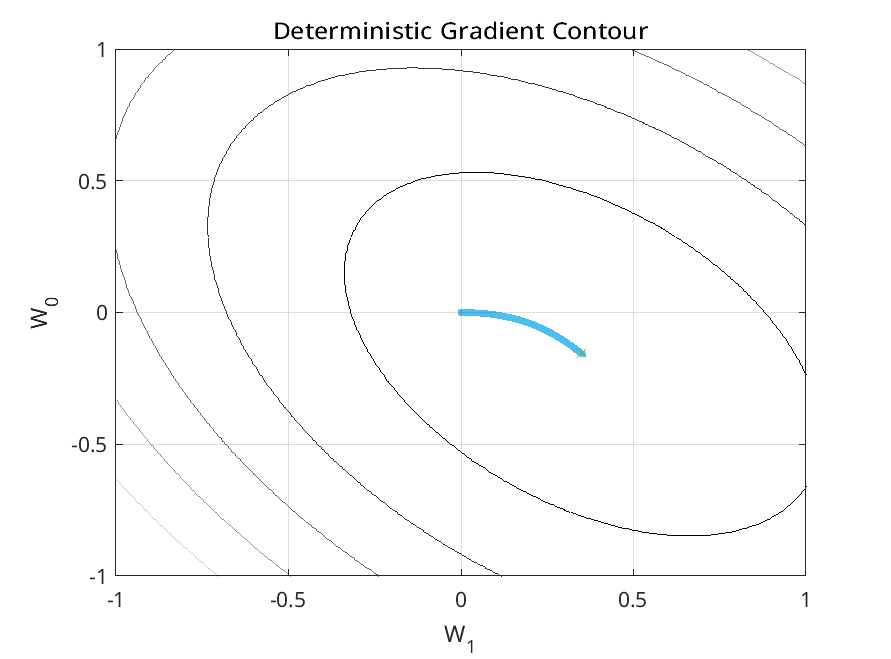
\includegraphics[width=0.75\textwidth]{figs/gradient_contour.png}
					\caption{Caminho de convergência na superficie MSE para o Gradiente Determinístico. $\text{Amostras} = 5000$, $M = 2$, $\mu = 10^{-3}$}
					\label{fig:gradient_contour}
				\end{figure}

				\begin{figure}[!ht]
					\centering
					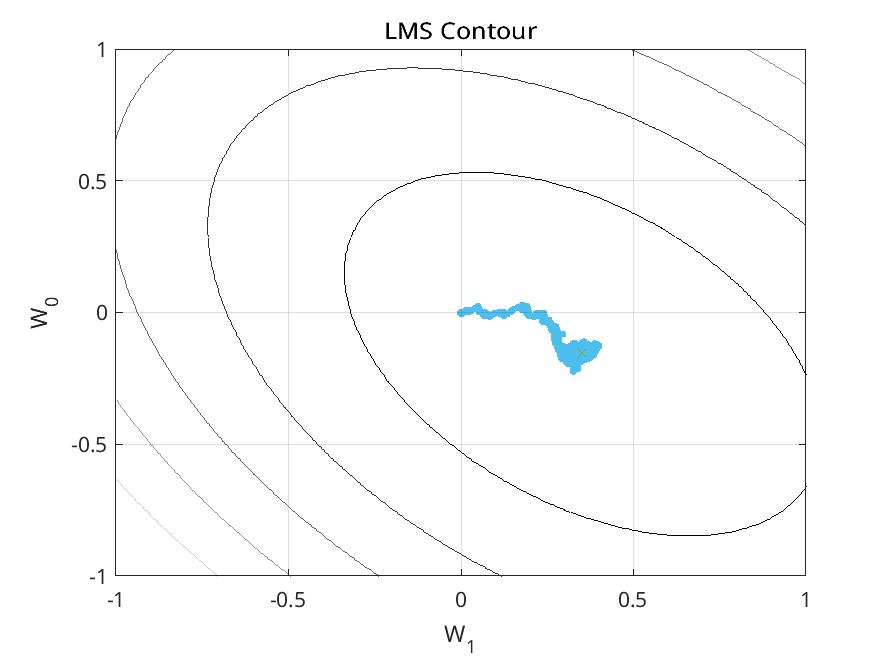
\includegraphics[width=0.75\textwidth]{figs/lms_contour.png}
					\caption{Caminho de convergência na superficie MSE para o LMS. $\text{Amostras} = 5000$, $M = 2$, $\mu = 10^{-3}$}
					\label{fig:lms_contour}
				\end{figure}

				\begin{figure}[!ht]
					\centering
					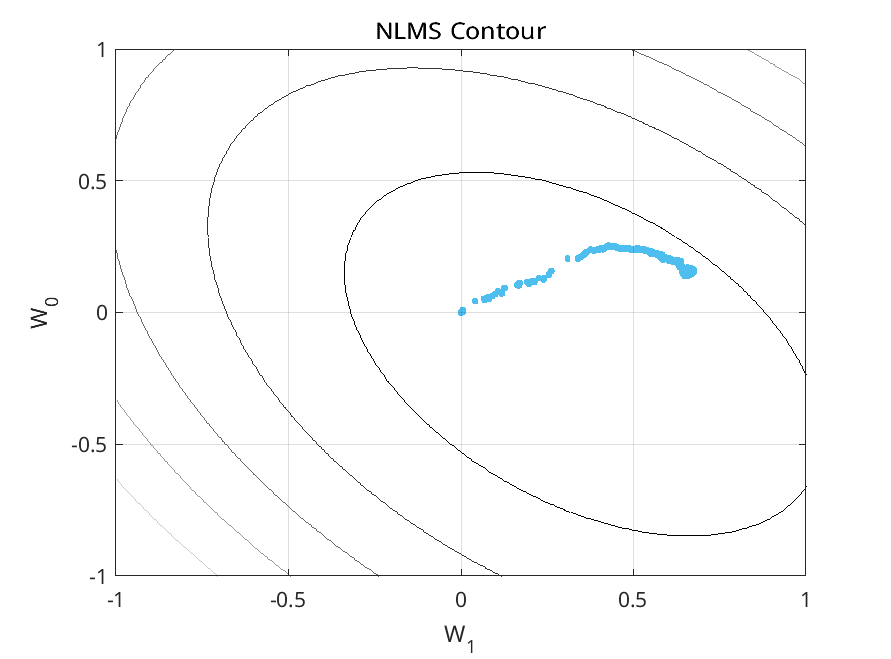
\includegraphics[width=0.75\textwidth]{figs/nlms_contour.png}
					\caption{Caminho de convergência na superficie MSE para o NLMS. $\text{Amostras} = 5000$, $M = 2$, $\mu = 10^{-3}$}
					\label{fig:nlms_contour}
				\end{figure}

				\begin{figure}[!ht]
					\centering
					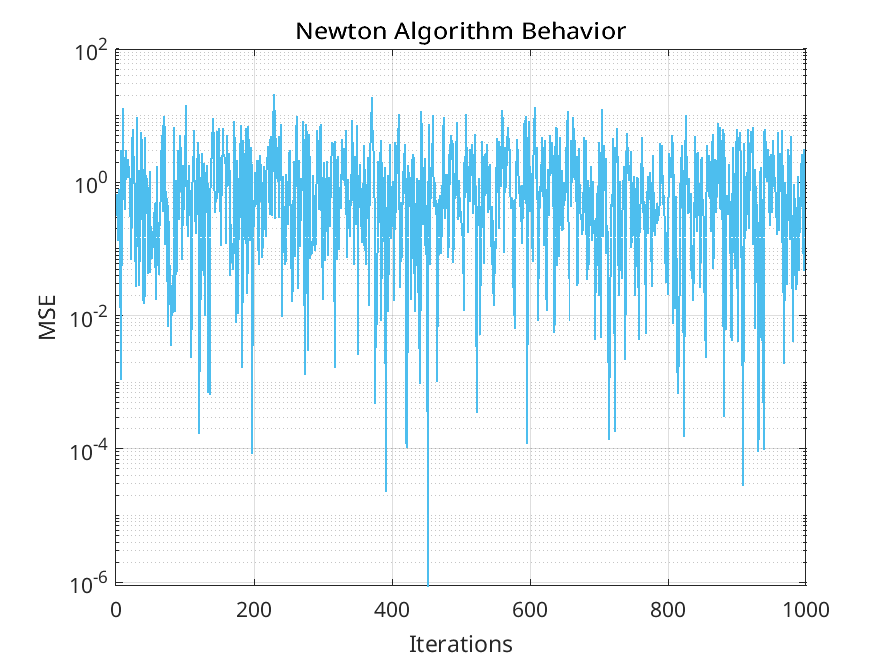
\includegraphics[width=0.75\textwidth]{figs/newton_mse.png}
					\caption{Caminho de convergência na superficie MSE para o Método de Newton. $\text{Amostras} = 5000$, $M = 2$, $\mu = 10^{-3}$}
					\label{fig:newton_mse}
				\end{figure}
				
				\begin{figure}[!ht]
					\centering
					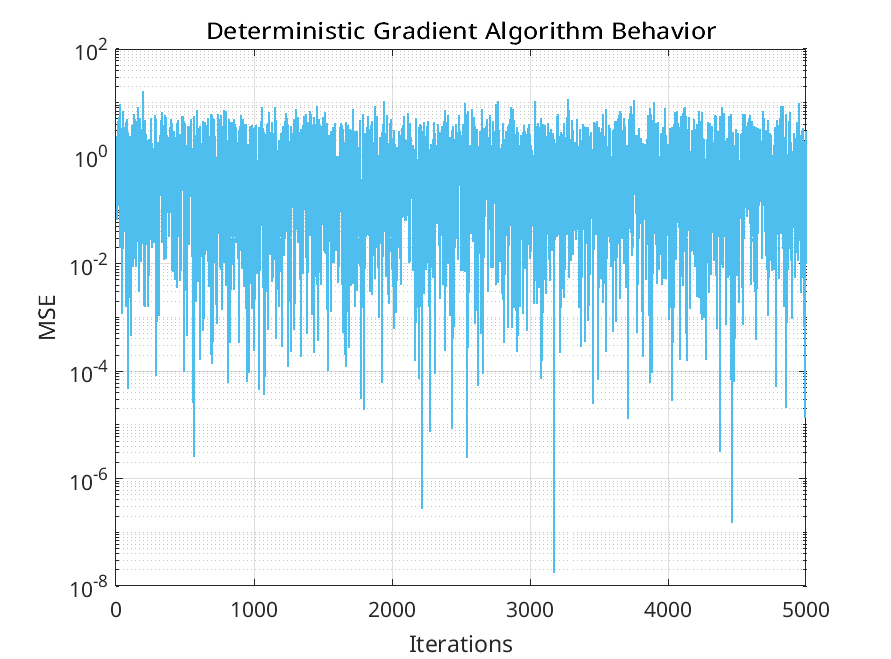
\includegraphics[width=0.75\textwidth]{figs/gradient_mse.png}
					\caption{Caminho de convergência na superficie MSE para o Gradiente Determinístico. $\text{Amostras} = 5000$, $M = 2$, $\mu = 10^{-3}$}
					\label{fig:gradient_mse}
				\end{figure}

				\begin{figure}[!ht]
					\centering
					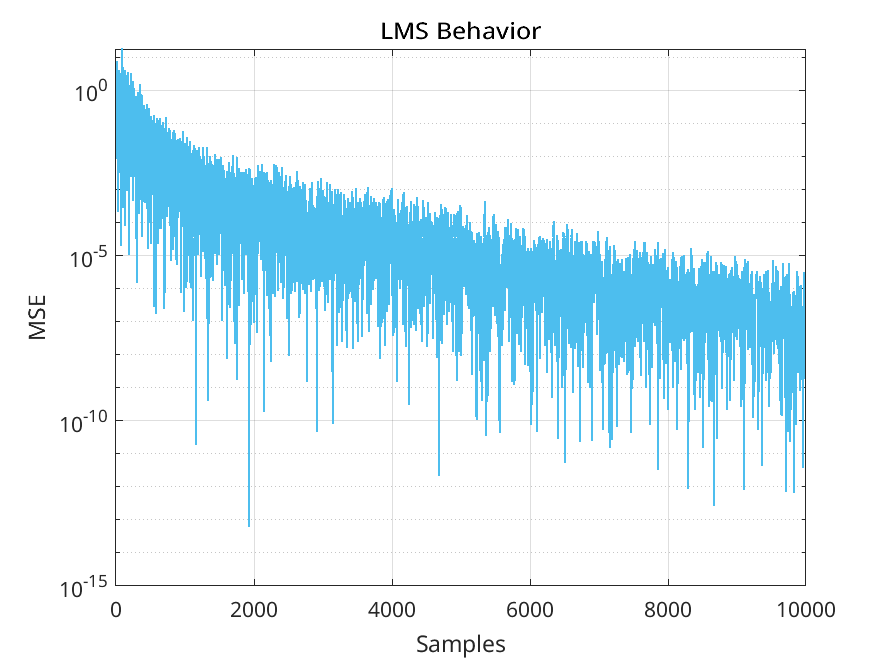
\includegraphics[width=0.75\textwidth]{figs/lms_mse.png}
					\caption{Caminho de convergência na superficie MSE para o LMS. $\text{Amostras}  = 5000$, $M = 2$, $\mu = 10^{-3}$}
					\label{fig:lms_mse}
				\end{figure}

				\begin{figure}[!ht]
					\centering
					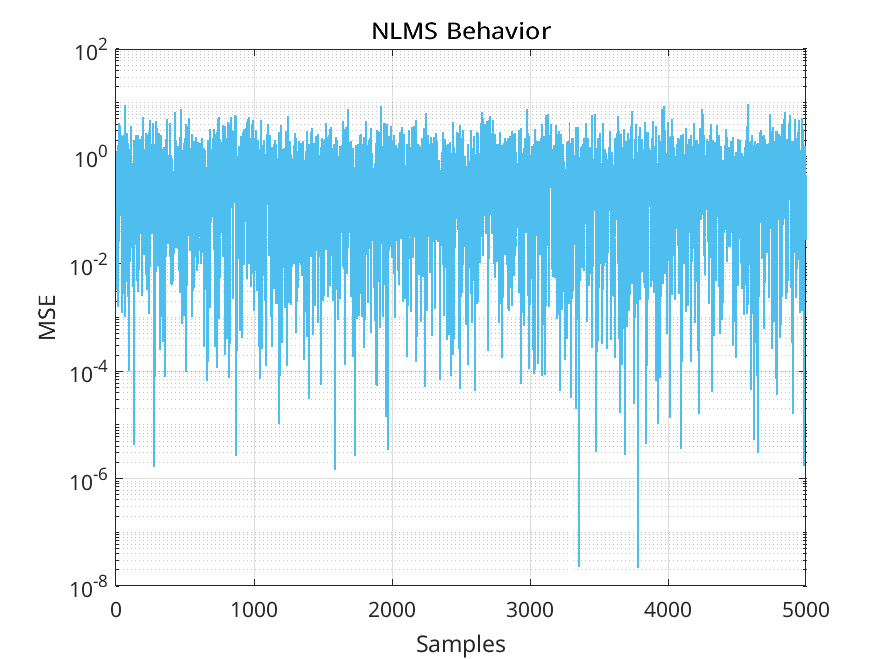
\includegraphics[width=0.75\textwidth]{figs/nlms_mse.png}
					\caption{Caminho de convergência na superficie MSE para o NLMS. $\text{Amostras} = 5000$, $M = 2$, $\mu = 10^{-3}$}
					\label{fig:nlms_mse}
				\end{figure}

				\begin{figure}[!ht]
					\centering
					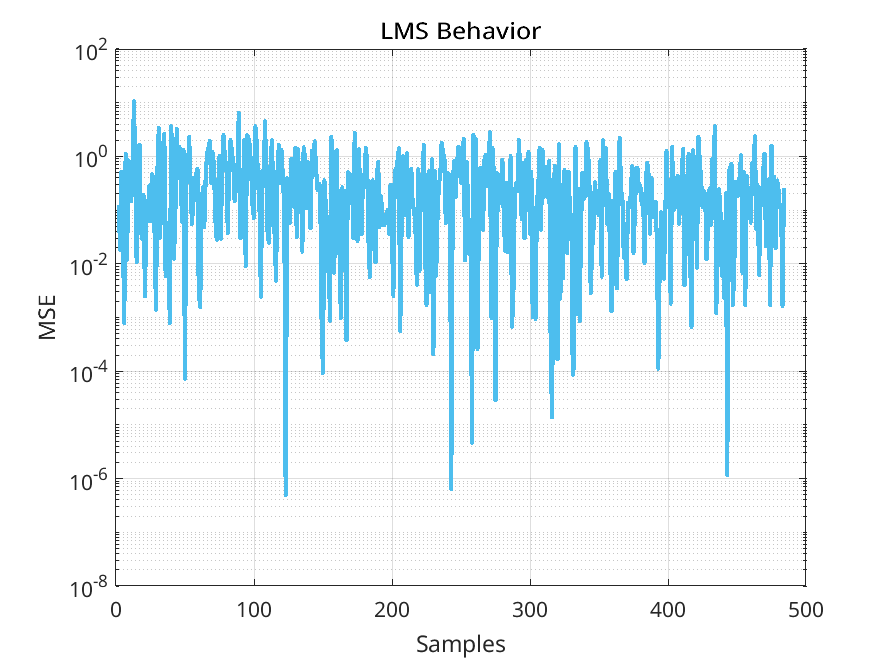
\includegraphics[width=0.75\textwidth]{figs/L3Q5_mu_2.png}
					\caption{$\text{Amostras} = 1500$, $M = 15$, $\mu = \frac{\mu_{\text{max}}}{2}$}
					\label{fig:mu_2}
				\end{figure}

				\begin{figure}[!ht]
					\centering
					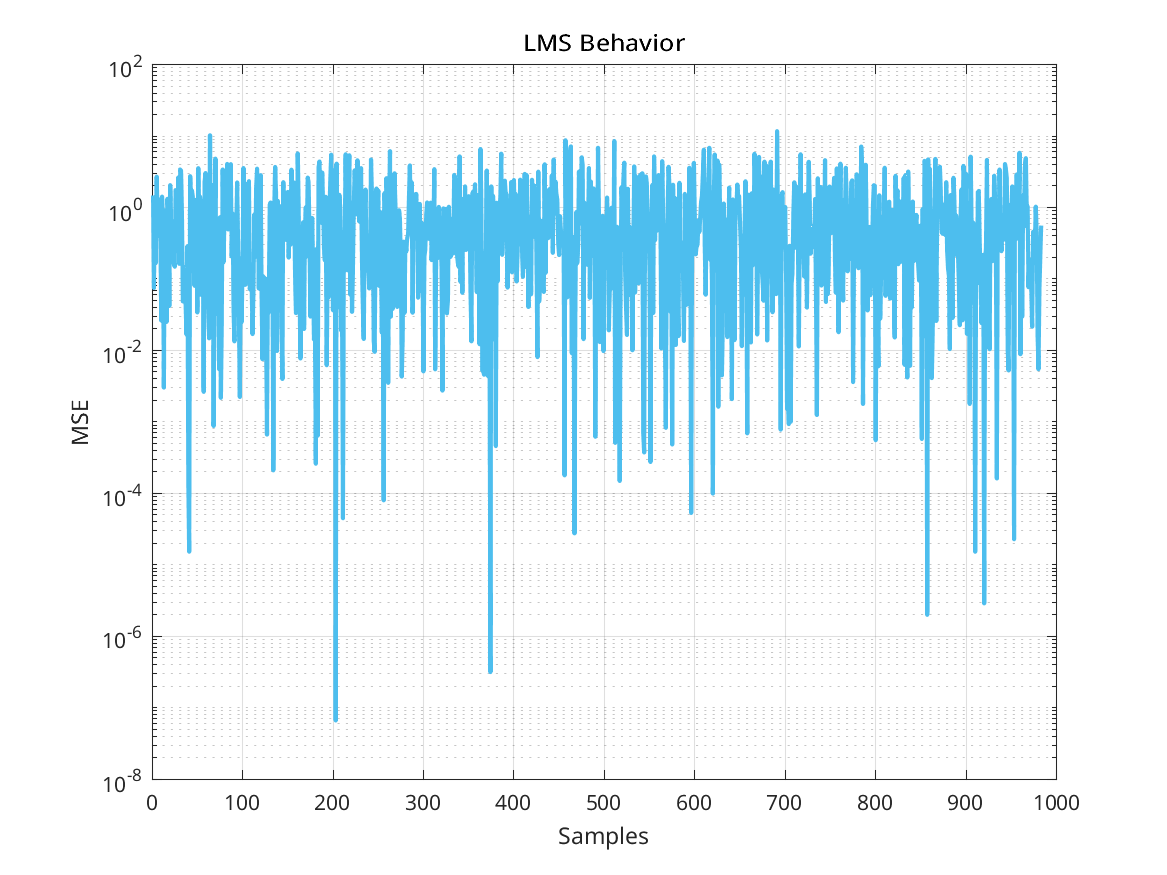
\includegraphics[width=0.75\textwidth]{figs/L3Q5_mu_10.png}
					\caption{$\text{Amostras} = 1500$, $M = 15$, $\mu = \frac{\mu_{\text{max}}}{10}$}
					\label{fig:mu_10}
				\end{figure}

				\begin{figure}[!ht]
					\centering
					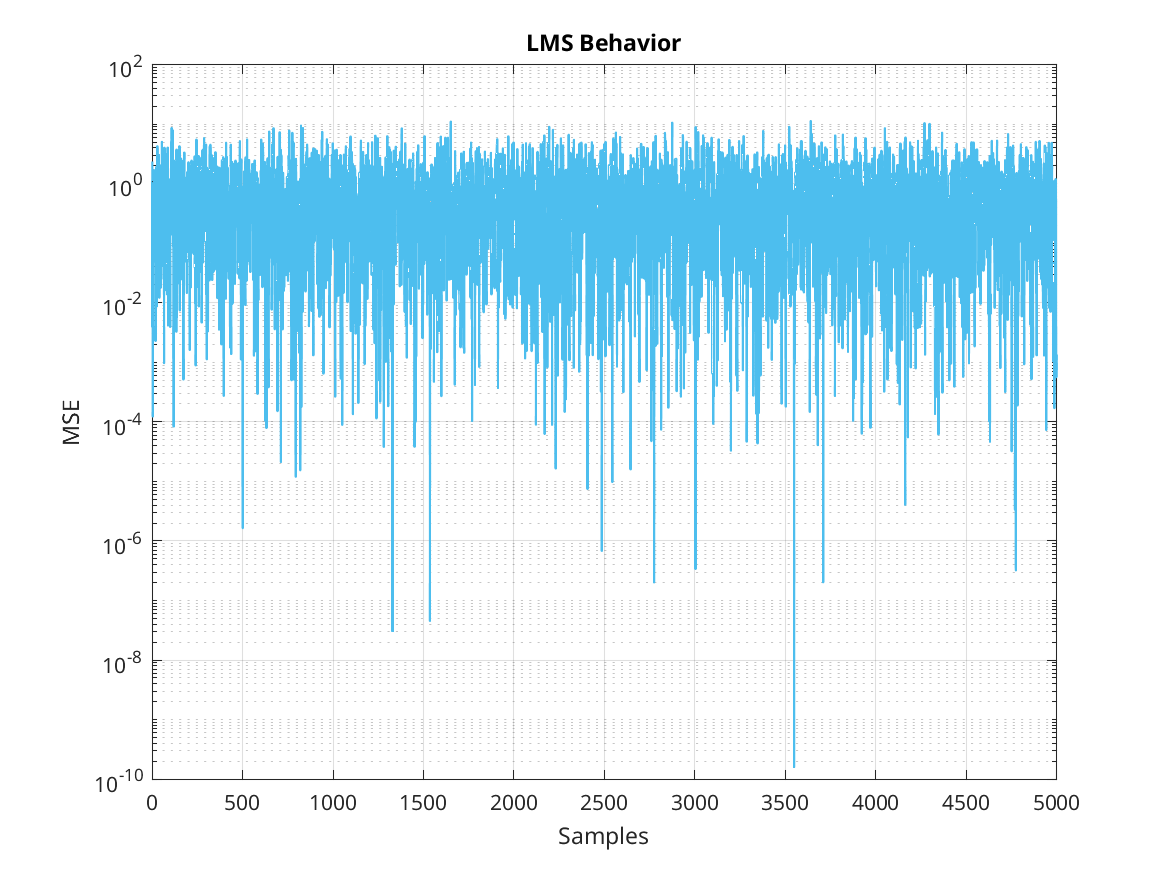
\includegraphics[width=0.75\textwidth]{figs/L3Q5_mu_50.png}
					\caption{$\text{Amostras} = 1500$, $M = 15$, $\mu = \frac{\mu_{\text{max}}}{50}$}
					\label{fig:mu_50}
				\end{figure}

				\begin{figure}[!ht]
					\centering
					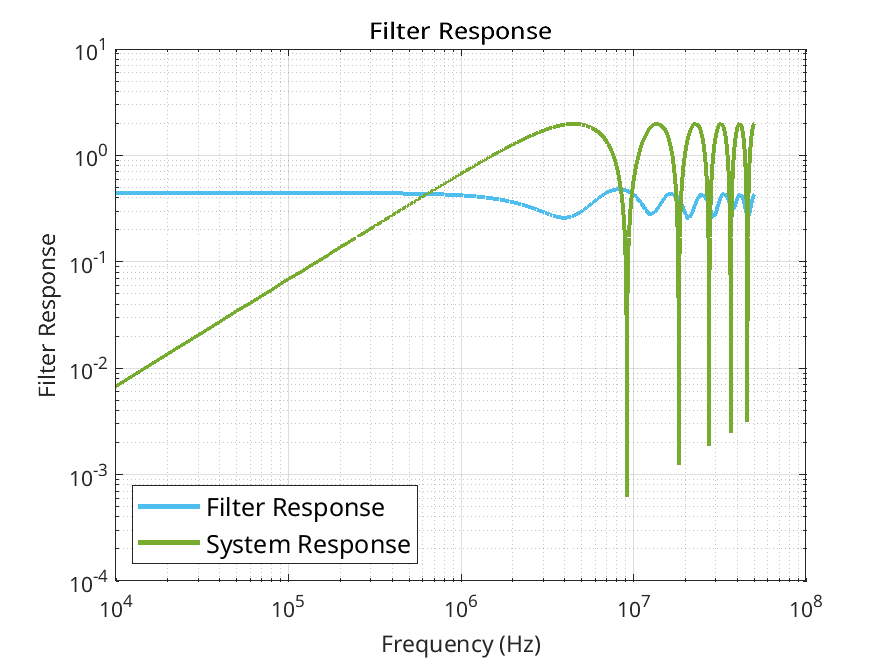
\includegraphics[width=0.75\textwidth]{figs/L3Q5_filter_response.png}
					\caption{$\text{Amostras} = 1500$, $M = 15$, $\mu = \frac{\mu_{\text{max}}}{2}$}
					\label{fig:filter_response}
				\end{figure}

				\begin{figure}[!ht]
					\centering
					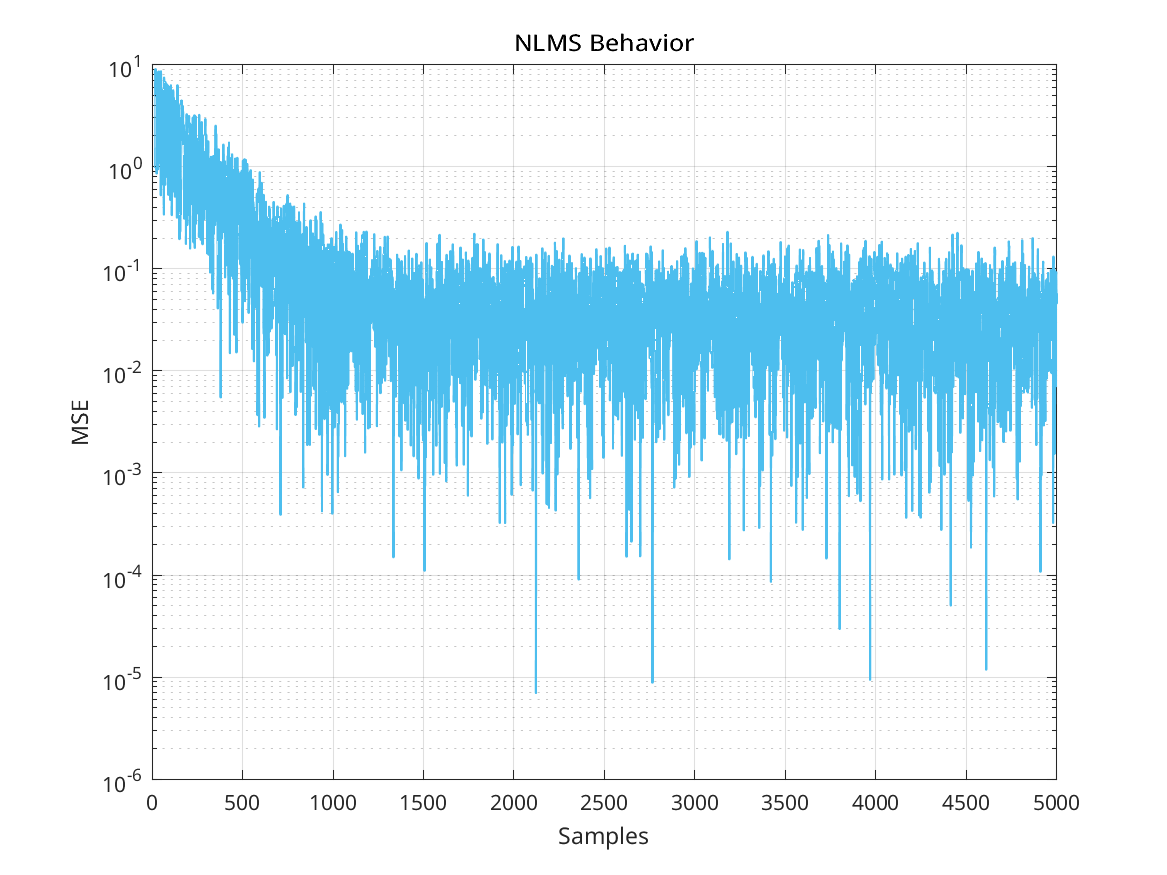
\includegraphics[width=0.75\textwidth]{figs/L3Q6_A_mse.png}
					\caption{$\text{Amostras} = 1500$, $M = 15$, $\mu = \frac{\mu_{\text{max}}}{2}$}
					\label{fig:L3Q6A1}
				\end{figure}

				\begin{figure}[!ht]
					\centering
					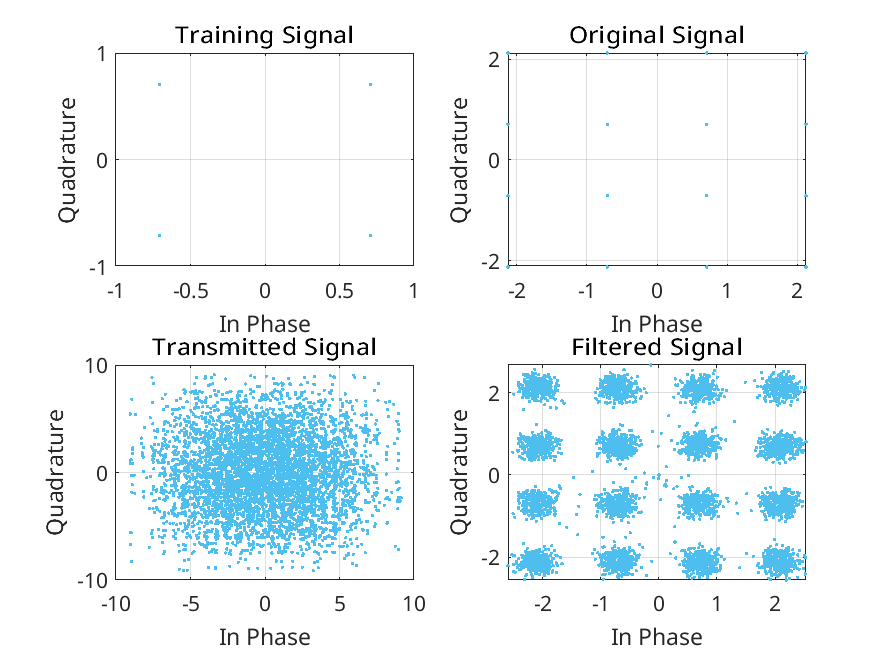
\includegraphics[width=0.75\textwidth]{figs/L3Q6_A_t.png}
					\caption{$\text{Amostras} = 5000$, $M = 15$, $\mu = 0.4$}
					\label{fig:L3Q6A2}
				\end{figure}

				\begin{figure}[!ht]
					\centering
					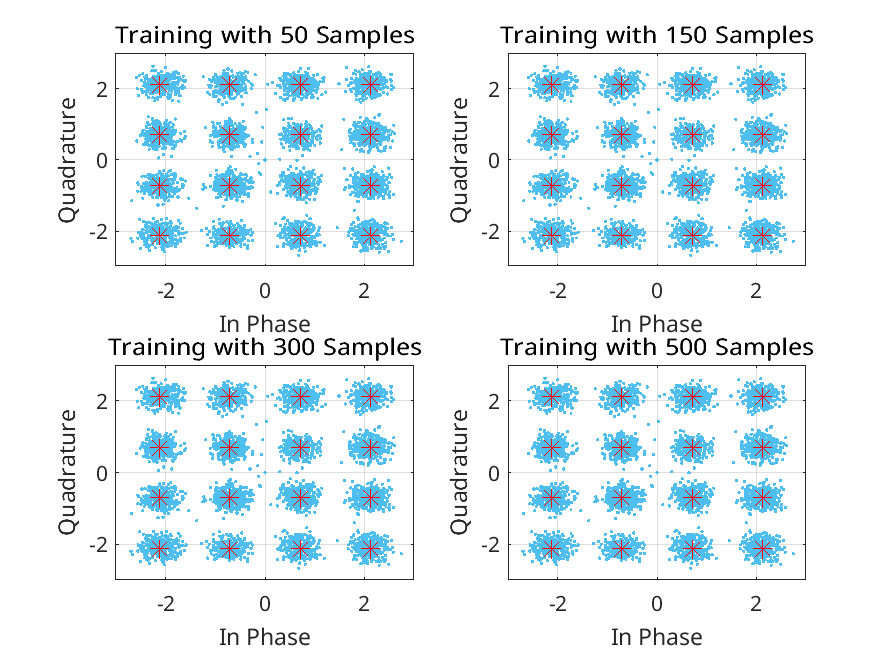
\includegraphics[width=0.75\textwidth]{figs/L3Q6_B_t.png}
					\caption{$\text{Amostras} = 5000$, $M = 15$, $\mu = 0.001$}
					\label{fig:L3Q6B}
				\end{figure}

				\begin{figure}[!ht]
					\centering
					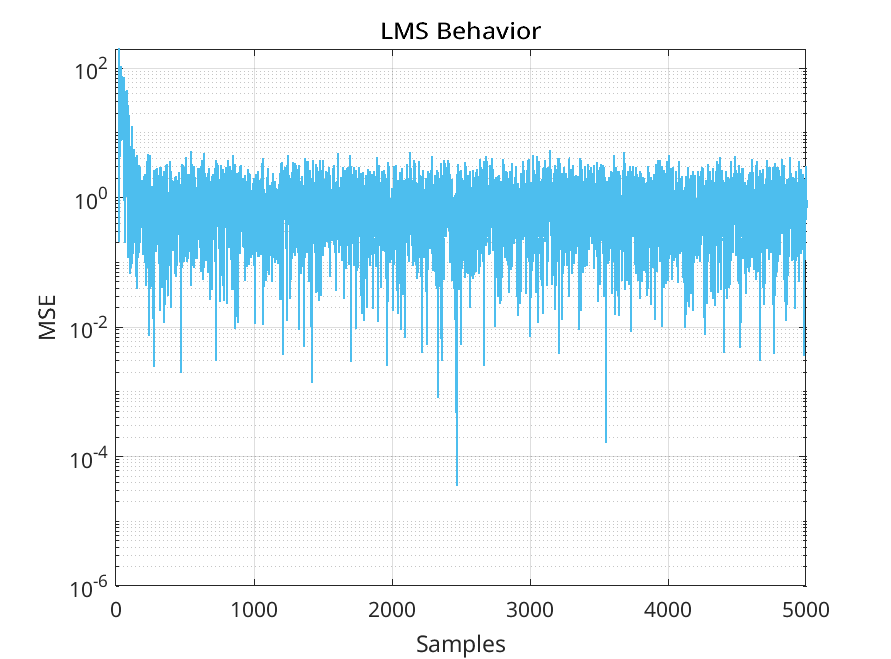
\includegraphics[width=0.75\textwidth]{figs/L3Q6_C_mse.png}
					\caption{$\text{Amostras} = 5000$, $M = 15$, $\mu = 0.4$}
					\label{fig:L3Q6C1}
				\end{figure}

				\begin{figure}[!ht]
					\centering
					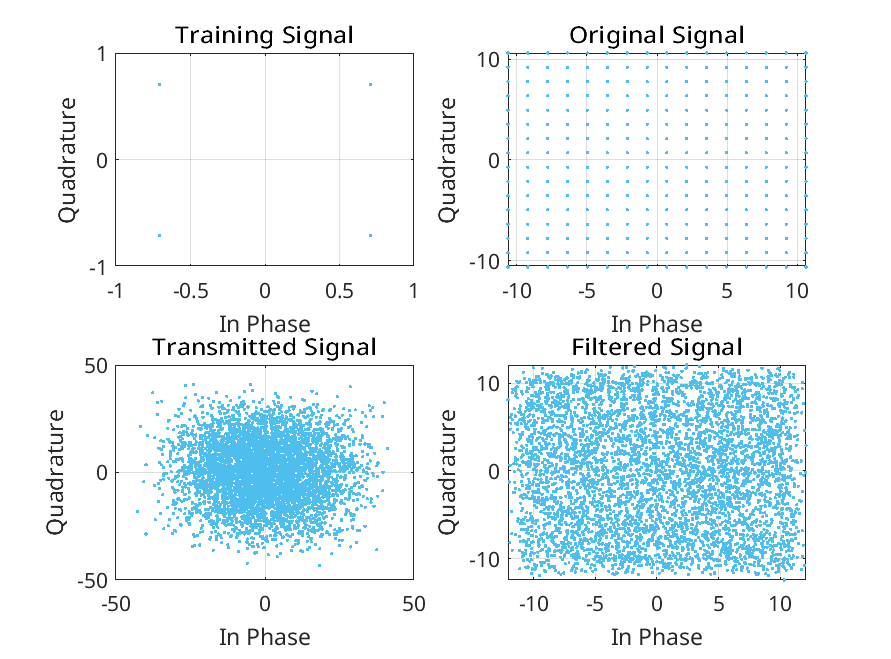
\includegraphics[width=0.75\textwidth]{figs/L3Q6_C_t.png}
					\caption{$\text{Amostras} = 5000$, $M = 15$, $\mu = 0.4$}
					\label{fig:L3Q6C2}
				\end{figure}

				\begin{figure}[!ht]
					\centering
					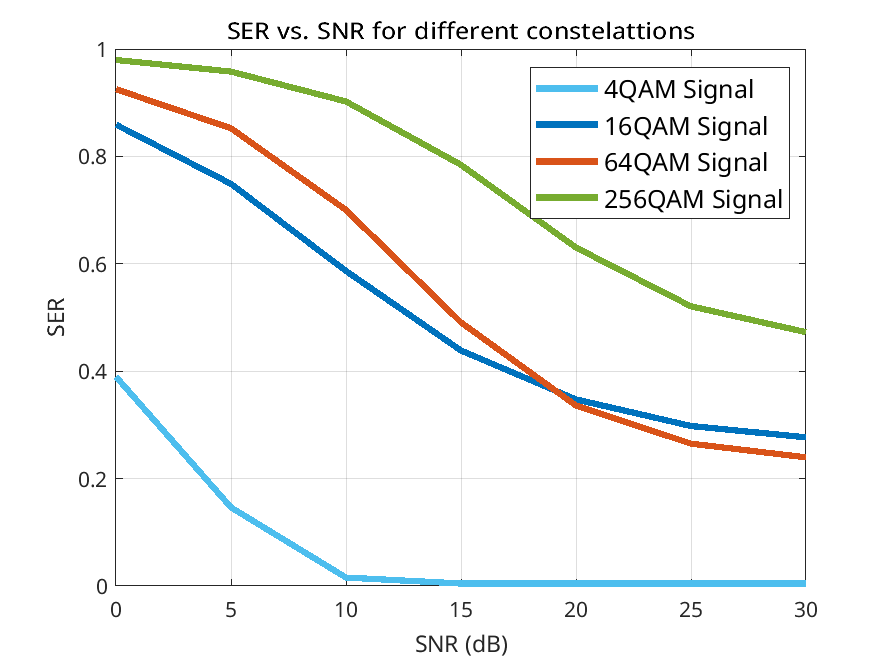
\includegraphics[width=0.75\textwidth]{figs/L3Q6_D_ser.png}
					\caption{$\text{Amostras} = 5000$, $M = 15$, $\mu = 0.4$}
					\label{fig:L3Q6D}
				\end{figure}

		\end{enumerate}
	
\end{document}

